\documentclass[twoside]{book}

% Packages required by doxygen
\usepackage{fixltx2e}
\usepackage{calc}
\usepackage{doxygen}
\usepackage[export]{adjustbox} % also loads graphicx
\usepackage{graphicx}
\usepackage[utf8]{inputenc}
\usepackage{makeidx}
\usepackage{multicol}
\usepackage{multirow}
\PassOptionsToPackage{warn}{textcomp}
\usepackage{textcomp}
\usepackage[nointegrals]{wasysym}
\usepackage[table]{xcolor}

% Font selection
\usepackage[T1]{fontenc}
\usepackage[scaled=.90]{helvet}
\usepackage{courier}
\usepackage{amssymb}
\usepackage{sectsty}
\renewcommand{\familydefault}{\sfdefault}
\allsectionsfont{%
  \fontseries{bc}\selectfont%
  \color{darkgray}%
}
\renewcommand{\DoxyLabelFont}{%
  \fontseries{bc}\selectfont%
  \color{darkgray}%
}
\newcommand{\+}{\discretionary{\mbox{\scriptsize$\hookleftarrow$}}{}{}}

% Page & text layout
\usepackage{geometry}
\geometry{%
  a4paper,%
  top=2.5cm,%
  bottom=2.5cm,%
  left=2.5cm,%
  right=2.5cm%
}
\tolerance=750
\hfuzz=15pt
\hbadness=750
\setlength{\emergencystretch}{15pt}
\setlength{\parindent}{0cm}
\setlength{\parskip}{3ex plus 2ex minus 2ex}
\makeatletter
\renewcommand{\paragraph}{%
  \@startsection{paragraph}{4}{0ex}{-1.0ex}{1.0ex}{%
    \normalfont\normalsize\bfseries\SS@parafont%
  }%
}
\renewcommand{\subparagraph}{%
  \@startsection{subparagraph}{5}{0ex}{-1.0ex}{1.0ex}{%
    \normalfont\normalsize\bfseries\SS@subparafont%
  }%
}
\makeatother

% Headers & footers
\usepackage{fancyhdr}
\pagestyle{fancyplain}
\fancyhead[LE]{\fancyplain{}{\bfseries\thepage}}
\fancyhead[CE]{\fancyplain{}{}}
\fancyhead[RE]{\fancyplain{}{\bfseries\leftmark}}
\fancyhead[LO]{\fancyplain{}{\bfseries\rightmark}}
\fancyhead[CO]{\fancyplain{}{}}
\fancyhead[RO]{\fancyplain{}{\bfseries\thepage}}
\fancyfoot[LE]{\fancyplain{}{}}
\fancyfoot[CE]{\fancyplain{}{}}
\fancyfoot[RE]{\fancyplain{}{\bfseries\scriptsize Generated by Doxygen }}
\fancyfoot[LO]{\fancyplain{}{\bfseries\scriptsize Generated by Doxygen }}
\fancyfoot[CO]{\fancyplain{}{}}
\fancyfoot[RO]{\fancyplain{}{}}
\renewcommand{\footrulewidth}{0.4pt}
\renewcommand{\chaptermark}[1]{%
  \markboth{#1}{}%
}
\renewcommand{\sectionmark}[1]{%
  \markright{\thesection\ #1}%
}

% Indices & bibliography
\usepackage{natbib}
\usepackage[titles]{tocloft}
\setcounter{tocdepth}{3}
\setcounter{secnumdepth}{5}
\makeindex

% Hyperlinks (required, but should be loaded last)
\usepackage{ifpdf}
\ifpdf
  \usepackage[pdftex,pagebackref=true]{hyperref}
\else
  \usepackage[ps2pdf,pagebackref=true]{hyperref}
\fi
\hypersetup{%
  colorlinks=true,%
  linkcolor=blue,%
  citecolor=blue,%
  unicode%
}

% Custom commands
\newcommand{\clearemptydoublepage}{%
  \newpage{\pagestyle{empty}\cleardoublepage}%
}

\usepackage{caption}
\captionsetup{labelsep=space,justification=centering,font={bf},singlelinecheck=off,skip=4pt,position=top}

%===== C O N T E N T S =====

\begin{document}

% Titlepage & ToC
\hypersetup{pageanchor=false,
             bookmarksnumbered=true,
             pdfencoding=unicode
            }
\pagenumbering{alph}
\begin{titlepage}
\vspace*{7cm}
\begin{center}%
{\Large Auto\+Cell }\\
\vspace*{1cm}
{\large Generated by Doxygen 1.8.14}\\
\end{center}
\end{titlepage}
\clearemptydoublepage
\pagenumbering{roman}
\tableofcontents
\clearemptydoublepage
\pagenumbering{arabic}
\hypersetup{pageanchor=true}

%--- Begin generated contents ---
\chapter{Hierarchical Index}
\section{Class Hierarchy}
This inheritance list is sorted roughly, but not completely, alphabetically\+:\begin{DoxyCompactList}
\item \contentsline{section}{Automate\+Exception}{\pageref{class_automate_exception}}{}
\item \contentsline{section}{Cell}{\pageref{class_cell}}{}
\item \contentsline{section}{Cellular\+Automata}{\pageref{class_cellular_automata}}{}
\item \contentsline{section}{Etat}{\pageref{class_etat}}{}
\item \contentsline{section}{Generateur\+Etat}{\pageref{class_generateur_etat}}{}
\begin{DoxyCompactList}
\item \contentsline{section}{Generateur\+Random}{\pageref{class_generateur_random}}{}
\item \contentsline{section}{Generateur\+Symetrie\+Axe\+Largeur}{\pageref{class_generateur_symetrie_axe_largeur}}{}
\end{DoxyCompactList}
\item \contentsline{section}{Transition\+Rule}{\pageref{class_transition_rule}}{}
\begin{DoxyCompactList}
\item \contentsline{section}{Transition\+Rule1D}{\pageref{class_transition_rule1_d}}{}
\begin{DoxyCompactList}
\item \contentsline{section}{Elementary\+Rule}{\pageref{class_elementary_rule}}{}
\end{DoxyCompactList}
\item \contentsline{section}{Transition\+Rule2D}{\pageref{class_transition_rule2_d}}{}
\begin{DoxyCompactList}
\item \contentsline{section}{Feu\+Foret}{\pageref{class_feu_foret}}{}
\item \contentsline{section}{Game\+Of\+Life}{\pageref{class_game_of_life}}{}
\end{DoxyCompactList}
\end{DoxyCompactList}
\item \contentsline{section}{Voisinage}{\pageref{class_voisinage}}{}
\begin{DoxyCompactList}
\item \contentsline{section}{Voisinage1D}{\pageref{class_voisinage1_d}}{}
\item \contentsline{section}{Voisinage2D}{\pageref{class_voisinage2_d}}{}
\begin{DoxyCompactList}
\item \contentsline{section}{Moore}{\pageref{class_moore}}{}
\item \contentsline{section}{Von\+Neumann}{\pageref{class_von_neumann}}{}
\end{DoxyCompactList}
\end{DoxyCompactList}
\end{DoxyCompactList}

\chapter{Class Index}
\section{Class List}
Here are the classes, structs, unions and interfaces with brief descriptions\+:\begin{DoxyCompactList}
\item\contentsline{section}{\mbox{\hyperlink{class_automate_exception}{Automate\+Exception}} }{\pageref{class_automate_exception}}{}
\item\contentsline{section}{\mbox{\hyperlink{class_cell}{Cell}} }{\pageref{class_cell}}{}
\item\contentsline{section}{\mbox{\hyperlink{class_cellular_automata}{Cellular\+Automata}} }{\pageref{class_cellular_automata}}{}
\item\contentsline{section}{\mbox{\hyperlink{class_elementary_rule}{Elementary\+Rule}} }{\pageref{class_elementary_rule}}{}
\item\contentsline{section}{\mbox{\hyperlink{class_etat}{Etat}} }{\pageref{class_etat}}{}
\item\contentsline{section}{\mbox{\hyperlink{class_feu_foret}{Feu\+Foret}} }{\pageref{class_feu_foret}}{}
\item\contentsline{section}{\mbox{\hyperlink{class_game_of_life}{Game\+Of\+Life}} }{\pageref{class_game_of_life}}{}
\item\contentsline{section}{\mbox{\hyperlink{class_generateur_etat}{Generateur\+Etat}} }{\pageref{class_generateur_etat}}{}
\item\contentsline{section}{\mbox{\hyperlink{class_generateur_random}{Generateur\+Random}} }{\pageref{class_generateur_random}}{}
\item\contentsline{section}{\mbox{\hyperlink{class_generateur_symetrie_axe_largeur}{Generateur\+Symetrie\+Axe\+Largeur}} }{\pageref{class_generateur_symetrie_axe_largeur}}{}
\item\contentsline{section}{\mbox{\hyperlink{class_moore}{Moore}} }{\pageref{class_moore}}{}
\item\contentsline{section}{\mbox{\hyperlink{class_transition_rule}{Transition\+Rule}} }{\pageref{class_transition_rule}}{}
\item\contentsline{section}{\mbox{\hyperlink{class_transition_rule1_d}{Transition\+Rule1D}} }{\pageref{class_transition_rule1_d}}{}
\item\contentsline{section}{\mbox{\hyperlink{class_transition_rule2_d}{Transition\+Rule2D}} }{\pageref{class_transition_rule2_d}}{}
\item\contentsline{section}{\mbox{\hyperlink{class_voisinage}{Voisinage}} }{\pageref{class_voisinage}}{}
\item\contentsline{section}{\mbox{\hyperlink{class_voisinage1_d}{Voisinage1D}} }{\pageref{class_voisinage1_d}}{}
\item\contentsline{section}{\mbox{\hyperlink{class_voisinage2_d}{Voisinage2D}} }{\pageref{class_voisinage2_d}}{}
\item\contentsline{section}{\mbox{\hyperlink{class_von_neumann}{Von\+Neumann}} }{\pageref{class_von_neumann}}{}
\end{DoxyCompactList}

\chapter{Class Documentation}
\hypertarget{class_automate_exception}{}\section{Automate\+Exception Class Reference}
\label{class_automate_exception}\index{Automate\+Exception@{Automate\+Exception}}
\subsection*{Public Member Functions}
\begin{DoxyCompactItemize}
\item 
\mbox{\Hypertarget{class_automate_exception_a324660f942b04229a4795cc80c3dbe82}\label{class_automate_exception_a324660f942b04229a4795cc80c3dbe82}} 
{\bfseries Automate\+Exception} (const std\+::string \&message)
\item 
\mbox{\Hypertarget{class_automate_exception_a7cd3843008b505a523231877bbf88699}\label{class_automate_exception_a7cd3843008b505a523231877bbf88699}} 
std\+::string {\bfseries get\+Info} () const
\end{DoxyCompactItemize}
\subsection*{Private Attributes}
\begin{DoxyCompactItemize}
\item 
\mbox{\Hypertarget{class_automate_exception_a016b50d51f7b0ff70ce26394e4004760}\label{class_automate_exception_a016b50d51f7b0ff70ce26394e4004760}} 
std\+::string {\bfseries info}
\end{DoxyCompactItemize}


The documentation for this class was generated from the following files\+:\begin{DoxyCompactItemize}
\item 
C\+:/\+Users/maxn0/git/\+L\+O21/\+Auto\+Cell/automateexception.\+h\item 
C\+:/\+Users/maxn0/git/\+L\+O21/\+Auto\+Cell/automateexception.\+cpp\end{DoxyCompactItemize}

\hypertarget{class_cell}{}\section{Référence de la classe Cell}
\label{class_cell}\index{Cell@{Cell}}


classe représentant une cellule \+: élément de base du programme  




{\ttfamily \#include $<$cell.\+h$>$}

\subsection*{Fonctions membres publiques}
\begin{DoxyCompactItemize}
\item 
std\+::vector$<$ \mbox{\hyperlink{class_cell}{Cell}} $\ast$ $>$ const  \& \mbox{\hyperlink{class_cell_a5c2a7b09dcb8afed0040ebdc4267408d}{Get\+Voisins}} () const
\begin{DoxyCompactList}\small\item\em Accesseur en lecture sur m\+\_\+voisins. \end{DoxyCompactList}\item 
int \mbox{\hyperlink{class_cell_a7640093c787979958fbb772e4fccdffa}{Get\+Etat}} () const
\begin{DoxyCompactList}\small\item\em Accesseur en lecture sur m\+\_\+etat. \end{DoxyCompactList}\item 
int \mbox{\hyperlink{class_cell_a3af5ea9b9e031151e16009b22118b07a}{GetX}} () const
\begin{DoxyCompactList}\small\item\em Accesseur en lecture sur m\+\_\+x. \end{DoxyCompactList}\item 
int \mbox{\hyperlink{class_cell_a3668c9664cadb1b94a632d497fa493c5}{GetY}} () const
\begin{DoxyCompactList}\small\item\em Accesseur en lecture sur m\+\_\+y. \end{DoxyCompactList}\item 
void \mbox{\hyperlink{class_cell_a33dac87ec7294fdb4c67b8b430ea0946}{Set\+Etat}} (int \mbox{\hyperlink{cell_8h_ae60adcb558b7f2142c3aa2dd94aaa535}{etat}})
\begin{DoxyCompactList}\small\item\em modification de l\textquotesingle{}etat \end{DoxyCompactList}\item 
void \mbox{\hyperlink{class_cell_aef5912d85e2ca3e034023fb0874896fa}{Ajouter\+Voisin}} (\mbox{\hyperlink{class_cell}{Cell}} $\ast$voisin)
\begin{DoxyCompactList}\small\item\em ajout d\textquotesingle{}un voisin dans le voisinage de la cellule \end{DoxyCompactList}\item 
void \mbox{\hyperlink{class_cell_a4f07be87bb04bdc457726c51f2c69bcc}{Clear\+Voisinage}} ()
\begin{DoxyCompactList}\small\item\em Suppression du voisinage. \end{DoxyCompactList}\end{DoxyCompactItemize}
\subsection*{Fonctions membres privées}
\begin{DoxyCompactItemize}
\item 
\mbox{\hyperlink{class_cell_a508f988fb5b1ef8358589363c1af3ee4}{$\sim$\+Cell}} ()=default
\begin{DoxyCompactList}\small\item\em Destructeur par défaut. \end{DoxyCompactList}\item 
\mbox{\hyperlink{class_cell_a394510643e8664cf12b5efaf5cb99f71}{Cell}} ()
\begin{DoxyCompactList}\small\item\em Constructeur. \end{DoxyCompactList}\item 
\mbox{\hyperlink{class_cell_abfff4b378d15d85506663df528762eaf}{Cell}} (int \mbox{\hyperlink{cell_8h_ae60adcb558b7f2142c3aa2dd94aaa535}{etat}}, int x, int y)
\begin{DoxyCompactList}\small\item\em Constructeur. \end{DoxyCompactList}\item 
\mbox{\hyperlink{class_cell_aff4c807938a63e9469c1547e7c087e0b}{Cell}} (\mbox{\hyperlink{class_cell}{Cell}} const \&c)=default
\begin{DoxyCompactList}\small\item\em Constructeur de recopie. \end{DoxyCompactList}\item 
void \mbox{\hyperlink{class_cell_a9aaedcce2daccb4aa070f870c1a207ed}{SetX}} (int x)
\begin{DoxyCompactList}\small\item\em modification de la position X \end{DoxyCompactList}\item 
void \mbox{\hyperlink{class_cell_a48afb0c8c8d1ebe3409b9a166dcd507d}{SetY}} (int y)
\begin{DoxyCompactList}\small\item\em modification de la position Y \end{DoxyCompactList}\item 
\mbox{\hyperlink{class_cell}{Cell}} \& \mbox{\hyperlink{class_cell_ac1f905d4cd626cc32963ab7a6f76634e}{operator=}} (\mbox{\hyperlink{class_cell}{Cell}} const \&c)=default
\begin{DoxyCompactList}\small\item\em surcharge de l\textquotesingle{}opérateur d\textquotesingle{}affectation (défaut) \end{DoxyCompactList}\end{DoxyCompactItemize}
\subsection*{Attributs privés}
\begin{DoxyCompactItemize}
\item 
int \mbox{\hyperlink{class_cell_a350cfee41db7450651de4e48543227c3}{m\+\_\+etat}}
\begin{DoxyCompactList}\small\item\em état (valeur) de la cellule. \end{DoxyCompactList}\item 
std\+::vector$<$ \mbox{\hyperlink{class_cell}{Cell}} $\ast$ $>$ \mbox{\hyperlink{class_cell_a7d781cbf0f2a5dffd13313b8eab86732}{m\+\_\+voisins}}
\begin{DoxyCompactList}\small\item\em vecteur de pointeurs sur les cellules voisines de la cellule \end{DoxyCompactList}\item 
int \mbox{\hyperlink{class_cell_ae38c546e6fd703965c8b62f750e68417}{m\+\_\+x}}
\begin{DoxyCompactList}\small\item\em position en ligne de la cellule \end{DoxyCompactList}\item 
int \mbox{\hyperlink{class_cell_a303c301e529e95ce1eadaf5b73ad41b2}{m\+\_\+y}}
\begin{DoxyCompactList}\small\item\em position en colonne de la cellule \end{DoxyCompactList}\end{DoxyCompactItemize}
\subsection*{Amis}
\begin{DoxyCompactItemize}
\item 
class \mbox{\hyperlink{class_cell_af495e82aa15594b628d4192e8ecb688b}{Etat}}
\end{DoxyCompactItemize}


\subsection{Description détaillée}
classe représentant une cellule \+: élément de base du programme 

Un objet \mbox{\hyperlink{class_cell}{Cell}} est une cellule qui fait nécessairement partie d\textquotesingle{}un objet \mbox{\hyperlink{class_etat}{Etat}} car seule \mbox{\hyperlink{class_etat}{Etat}} peut construire des objets \mbox{\hyperlink{class_cell}{Cell}}. Une cellule est caractérisée par sa position, son état (sa valeur), un voisinage. 

\subsection{Documentation des constructeurs et destructeur}
\mbox{\Hypertarget{class_cell_a508f988fb5b1ef8358589363c1af3ee4}\label{class_cell_a508f988fb5b1ef8358589363c1af3ee4}} 
\index{Cell@{Cell}!````~Cell@{$\sim$\+Cell}}
\index{````~Cell@{$\sim$\+Cell}!Cell@{Cell}}
\subsubsection{\texorpdfstring{$\sim$\+Cell()}{~Cell()}}
{\footnotesize\ttfamily Cell\+::$\sim$\+Cell (\begin{DoxyParamCaption}{ }\end{DoxyParamCaption})\hspace{0.3cm}{\ttfamily [private]}, {\ttfamily [default]}}



Destructeur par défaut. 

\mbox{\Hypertarget{class_cell_a394510643e8664cf12b5efaf5cb99f71}\label{class_cell_a394510643e8664cf12b5efaf5cb99f71}} 
\index{Cell@{Cell}!Cell@{Cell}}
\index{Cell@{Cell}!Cell@{Cell}}
\subsubsection{\texorpdfstring{Cell()}{Cell()}\hspace{0.1cm}{\footnotesize\ttfamily [1/3]}}
{\footnotesize\ttfamily Cell\+::\+Cell (\begin{DoxyParamCaption}{ }\end{DoxyParamCaption})\hspace{0.3cm}{\ttfamily [inline]}, {\ttfamily [private]}}



Constructeur. 

Constructeur par défault de la classe \mbox{\hyperlink{class_cell}{Cell}} \+: X, Y et l\textquotesingle{}état sont initialisés à 0. Seule la classe \mbox{\hyperlink{class_etat}{Etat}} peut construire des \mbox{\hyperlink{class_cell}{Cell}}. \mbox{\Hypertarget{class_cell_abfff4b378d15d85506663df528762eaf}\label{class_cell_abfff4b378d15d85506663df528762eaf}} 
\index{Cell@{Cell}!Cell@{Cell}}
\index{Cell@{Cell}!Cell@{Cell}}
\subsubsection{\texorpdfstring{Cell()}{Cell()}\hspace{0.1cm}{\footnotesize\ttfamily [2/3]}}
{\footnotesize\ttfamily Cell\+::\+Cell (\begin{DoxyParamCaption}\item[{int}]{etat,  }\item[{int}]{x,  }\item[{int}]{y }\end{DoxyParamCaption})\hspace{0.3cm}{\ttfamily [inline]}, {\ttfamily [private]}}



Constructeur. 

Constructeur de la classe \mbox{\hyperlink{class_cell}{Cell}}. Seule la classe \mbox{\hyperlink{class_etat}{Etat}} peut construire des \mbox{\hyperlink{class_cell}{Cell}}.


\begin{DoxyParams}{Paramètres}
{\em etat} & \+: valeur prise par la cellule \\
\hline
{\em x,y} & \+: positions \\
\hline
\end{DoxyParams}
\mbox{\Hypertarget{class_cell_aff4c807938a63e9469c1547e7c087e0b}\label{class_cell_aff4c807938a63e9469c1547e7c087e0b}} 
\index{Cell@{Cell}!Cell@{Cell}}
\index{Cell@{Cell}!Cell@{Cell}}
\subsubsection{\texorpdfstring{Cell()}{Cell()}\hspace{0.1cm}{\footnotesize\ttfamily [3/3]}}
{\footnotesize\ttfamily Cell\+::\+Cell (\begin{DoxyParamCaption}\item[{\mbox{\hyperlink{class_cell}{Cell}} const \&}]{c }\end{DoxyParamCaption})\hspace{0.3cm}{\ttfamily [private]}, {\ttfamily [default]}}



Constructeur de recopie. 

Constructeur de recopie de la classe \mbox{\hyperlink{class_cell}{Cell}}. Seule la classe \mbox{\hyperlink{class_etat}{Etat}} peut construire des \mbox{\hyperlink{class_cell}{Cell}}. 
\begin{DoxyParams}{Paramètres}
{\em c} & \+: référence sur la \mbox{\hyperlink{class_cell}{Cell}} qu\textquotesingle{}on souhaite copier \\
\hline
\end{DoxyParams}


\subsection{Documentation des fonctions membres}
\mbox{\Hypertarget{class_cell_aef5912d85e2ca3e034023fb0874896fa}\label{class_cell_aef5912d85e2ca3e034023fb0874896fa}} 
\index{Cell@{Cell}!Ajouter\+Voisin@{Ajouter\+Voisin}}
\index{Ajouter\+Voisin@{Ajouter\+Voisin}!Cell@{Cell}}
\subsubsection{\texorpdfstring{Ajouter\+Voisin()}{AjouterVoisin()}}
{\footnotesize\ttfamily void Cell\+::\+Ajouter\+Voisin (\begin{DoxyParamCaption}\item[{\mbox{\hyperlink{class_cell}{Cell}} $\ast$}]{voisin }\end{DoxyParamCaption})}



ajout d\textquotesingle{}un voisin dans le voisinage de la cellule 


\begin{DoxyParams}{Paramètres}
{\em voisin} & = pointeur sur la cellule voisine à ajouter \\
\hline
\end{DoxyParams}
\mbox{\Hypertarget{class_cell_a4f07be87bb04bdc457726c51f2c69bcc}\label{class_cell_a4f07be87bb04bdc457726c51f2c69bcc}} 
\index{Cell@{Cell}!Clear\+Voisinage@{Clear\+Voisinage}}
\index{Clear\+Voisinage@{Clear\+Voisinage}!Cell@{Cell}}
\subsubsection{\texorpdfstring{Clear\+Voisinage()}{ClearVoisinage()}}
{\footnotesize\ttfamily void Cell\+::\+Clear\+Voisinage (\begin{DoxyParamCaption}{ }\end{DoxyParamCaption})\hspace{0.3cm}{\ttfamily [inline]}}



Suppression du voisinage. 

\mbox{\Hypertarget{class_cell_a7640093c787979958fbb772e4fccdffa}\label{class_cell_a7640093c787979958fbb772e4fccdffa}} 
\index{Cell@{Cell}!Get\+Etat@{Get\+Etat}}
\index{Get\+Etat@{Get\+Etat}!Cell@{Cell}}
\subsubsection{\texorpdfstring{Get\+Etat()}{GetEtat()}}
{\footnotesize\ttfamily int Cell\+::\+Get\+Etat (\begin{DoxyParamCaption}{ }\end{DoxyParamCaption}) const\hspace{0.3cm}{\ttfamily [inline]}}



Accesseur en lecture sur m\+\_\+etat. 

\begin{DoxyReturn}{Renvoie}
etat de la cellule 
\end{DoxyReturn}
\mbox{\Hypertarget{class_cell_a5c2a7b09dcb8afed0040ebdc4267408d}\label{class_cell_a5c2a7b09dcb8afed0040ebdc4267408d}} 
\index{Cell@{Cell}!Get\+Voisins@{Get\+Voisins}}
\index{Get\+Voisins@{Get\+Voisins}!Cell@{Cell}}
\subsubsection{\texorpdfstring{Get\+Voisins()}{GetVoisins()}}
{\footnotesize\ttfamily std\+::vector$<$\mbox{\hyperlink{class_cell}{Cell}}$\ast$$>$ const\& Cell\+::\+Get\+Voisins (\begin{DoxyParamCaption}{ }\end{DoxyParamCaption}) const\hspace{0.3cm}{\ttfamily [inline]}}



Accesseur en lecture sur m\+\_\+voisins. 

Méthode permettant de récupérer une référence const sur l\textquotesingle{}ensemble des voisins d\textquotesingle{}une cellule. \begin{DoxyReturn}{Renvoie}
référence const sur le voisinage de la cellule qui est un vector de pointeurs de type \mbox{\hyperlink{class_cell}{Cell}} pointant chacun sur une cellule voisine de la cellule. 
\end{DoxyReturn}
\mbox{\Hypertarget{class_cell_a3af5ea9b9e031151e16009b22118b07a}\label{class_cell_a3af5ea9b9e031151e16009b22118b07a}} 
\index{Cell@{Cell}!GetX@{GetX}}
\index{GetX@{GetX}!Cell@{Cell}}
\subsubsection{\texorpdfstring{Get\+X()}{GetX()}}
{\footnotesize\ttfamily int Cell\+::\+GetX (\begin{DoxyParamCaption}{ }\end{DoxyParamCaption}) const\hspace{0.3cm}{\ttfamily [inline]}}



Accesseur en lecture sur m\+\_\+x. 

\begin{DoxyReturn}{Renvoie}
position en X (ligne) 
\end{DoxyReturn}
\mbox{\Hypertarget{class_cell_a3668c9664cadb1b94a632d497fa493c5}\label{class_cell_a3668c9664cadb1b94a632d497fa493c5}} 
\index{Cell@{Cell}!GetY@{GetY}}
\index{GetY@{GetY}!Cell@{Cell}}
\subsubsection{\texorpdfstring{Get\+Y()}{GetY()}}
{\footnotesize\ttfamily int Cell\+::\+GetY (\begin{DoxyParamCaption}{ }\end{DoxyParamCaption}) const\hspace{0.3cm}{\ttfamily [inline]}}



Accesseur en lecture sur m\+\_\+y. 

\begin{DoxyReturn}{Renvoie}
position en Y (colonne) 
\end{DoxyReturn}
\mbox{\Hypertarget{class_cell_ac1f905d4cd626cc32963ab7a6f76634e}\label{class_cell_ac1f905d4cd626cc32963ab7a6f76634e}} 
\index{Cell@{Cell}!operator=@{operator=}}
\index{operator=@{operator=}!Cell@{Cell}}
\subsubsection{\texorpdfstring{operator=()}{operator=()}}
{\footnotesize\ttfamily \mbox{\hyperlink{class_cell}{Cell}}\& Cell\+::operator= (\begin{DoxyParamCaption}\item[{\mbox{\hyperlink{class_cell}{Cell}} const \&}]{c }\end{DoxyParamCaption})\hspace{0.3cm}{\ttfamily [private]}, {\ttfamily [default]}}



surcharge de l\textquotesingle{}opérateur d\textquotesingle{}affectation (défaut) 


\begin{DoxyParams}{Paramètres}
{\em c} & \+: référence sur la cellule qui va nous servir à affecter la cellule courante \\
\hline
\end{DoxyParams}
\mbox{\Hypertarget{class_cell_a33dac87ec7294fdb4c67b8b430ea0946}\label{class_cell_a33dac87ec7294fdb4c67b8b430ea0946}} 
\index{Cell@{Cell}!Set\+Etat@{Set\+Etat}}
\index{Set\+Etat@{Set\+Etat}!Cell@{Cell}}
\subsubsection{\texorpdfstring{Set\+Etat()}{SetEtat()}}
{\footnotesize\ttfamily void Cell\+::\+Set\+Etat (\begin{DoxyParamCaption}\item[{int}]{etat }\end{DoxyParamCaption})}



modification de l\textquotesingle{}etat 


\begin{DoxyParams}{Paramètres}
{\em etat} & \+: valeur prise par la cellule \\
\hline
\end{DoxyParams}
\mbox{\Hypertarget{class_cell_a9aaedcce2daccb4aa070f870c1a207ed}\label{class_cell_a9aaedcce2daccb4aa070f870c1a207ed}} 
\index{Cell@{Cell}!SetX@{SetX}}
\index{SetX@{SetX}!Cell@{Cell}}
\subsubsection{\texorpdfstring{Set\+X()}{SetX()}}
{\footnotesize\ttfamily void Cell\+::\+SetX (\begin{DoxyParamCaption}\item[{int}]{x }\end{DoxyParamCaption})\hspace{0.3cm}{\ttfamily [private]}}



modification de la position X 

accesseur en écriture sur m\+\_\+x. Seule la classe \mbox{\hyperlink{class_etat}{Etat}} peut l\textquotesingle{}utiliser car il est illogique d\textquotesingle{}affecter une position X en dehors d\textquotesingle{}une grille. (Cet accesseur n\textquotesingle{}a pas grand intérêt car la classe \mbox{\hyperlink{class_etat}{Etat}} pourrait modifier m\+\_\+x directement vu que c\textquotesingle{}est une classe amie, mais nous avons pris la décision d\textquotesingle{}en faire une classe amie plus tard donc nous l\textquotesingle{}avons laissé afin de ne pas remodifier le code de la classe \mbox{\hyperlink{class_etat}{Etat}}) 
\begin{DoxyParams}{Paramètres}
{\em x} & \+: ligne \\
\hline
\end{DoxyParams}
\mbox{\Hypertarget{class_cell_a48afb0c8c8d1ebe3409b9a166dcd507d}\label{class_cell_a48afb0c8c8d1ebe3409b9a166dcd507d}} 
\index{Cell@{Cell}!SetY@{SetY}}
\index{SetY@{SetY}!Cell@{Cell}}
\subsubsection{\texorpdfstring{Set\+Y()}{SetY()}}
{\footnotesize\ttfamily void Cell\+::\+SetY (\begin{DoxyParamCaption}\item[{int}]{y }\end{DoxyParamCaption})\hspace{0.3cm}{\ttfamily [private]}}



modification de la position Y 

accesseur en écriture sur m\+\_\+y. Seule la classe \mbox{\hyperlink{class_etat}{Etat}} peut l\textquotesingle{}utiliser car il est illogique d\textquotesingle{}affecter une position Y en dehors d\textquotesingle{}une grille. (Cet accesseur n\textquotesingle{}a pas grand intérêt car la classe \mbox{\hyperlink{class_etat}{Etat}} pourrait modifier m\+\_\+y directement vu que c\textquotesingle{}est une classe amie, mais nous avons pris la décision d\textquotesingle{}en faire une classe amie plus tard donc nous l\textquotesingle{}avons laissé afin de ne pas remodifier le code de la classe \mbox{\hyperlink{class_etat}{Etat}}) 
\begin{DoxyParams}{Paramètres}
{\em y} & \+: colonne \\
\hline
\end{DoxyParams}


\subsection{Documentation des fonctions amies et associées}
\mbox{\Hypertarget{class_cell_af495e82aa15594b628d4192e8ecb688b}\label{class_cell_af495e82aa15594b628d4192e8ecb688b}} 
\index{Cell@{Cell}!Etat@{Etat}}
\index{Etat@{Etat}!Cell@{Cell}}
\subsubsection{\texorpdfstring{Etat}{Etat}}
{\footnotesize\ttfamily friend class \mbox{\hyperlink{class_etat}{Etat}}\hspace{0.3cm}{\ttfamily [friend]}}



\subsection{Documentation des données membres}
\mbox{\Hypertarget{class_cell_a350cfee41db7450651de4e48543227c3}\label{class_cell_a350cfee41db7450651de4e48543227c3}} 
\index{Cell@{Cell}!m\+\_\+etat@{m\+\_\+etat}}
\index{m\+\_\+etat@{m\+\_\+etat}!Cell@{Cell}}
\subsubsection{\texorpdfstring{m\+\_\+etat}{m\_etat}}
{\footnotesize\ttfamily int Cell\+::m\+\_\+etat\hspace{0.3cm}{\ttfamily [private]}}



état (valeur) de la cellule. 

\mbox{\Hypertarget{class_cell_a7d781cbf0f2a5dffd13313b8eab86732}\label{class_cell_a7d781cbf0f2a5dffd13313b8eab86732}} 
\index{Cell@{Cell}!m\+\_\+voisins@{m\+\_\+voisins}}
\index{m\+\_\+voisins@{m\+\_\+voisins}!Cell@{Cell}}
\subsubsection{\texorpdfstring{m\+\_\+voisins}{m\_voisins}}
{\footnotesize\ttfamily std\+::vector$<$\mbox{\hyperlink{class_cell}{Cell}}$\ast$$>$ Cell\+::m\+\_\+voisins\hspace{0.3cm}{\ttfamily [private]}}



vecteur de pointeurs sur les cellules voisines de la cellule 

\mbox{\Hypertarget{class_cell_ae38c546e6fd703965c8b62f750e68417}\label{class_cell_ae38c546e6fd703965c8b62f750e68417}} 
\index{Cell@{Cell}!m\+\_\+x@{m\+\_\+x}}
\index{m\+\_\+x@{m\+\_\+x}!Cell@{Cell}}
\subsubsection{\texorpdfstring{m\+\_\+x}{m\_x}}
{\footnotesize\ttfamily int Cell\+::m\+\_\+x\hspace{0.3cm}{\ttfamily [private]}}



position en ligne de la cellule 

\mbox{\Hypertarget{class_cell_a303c301e529e95ce1eadaf5b73ad41b2}\label{class_cell_a303c301e529e95ce1eadaf5b73ad41b2}} 
\index{Cell@{Cell}!m\+\_\+y@{m\+\_\+y}}
\index{m\+\_\+y@{m\+\_\+y}!Cell@{Cell}}
\subsubsection{\texorpdfstring{m\+\_\+y}{m\_y}}
{\footnotesize\ttfamily int Cell\+::m\+\_\+y\hspace{0.3cm}{\ttfamily [private]}}



position en colonne de la cellule 



La documentation de cette classe a été générée à partir des fichiers suivants \+:\begin{DoxyCompactItemize}
\item 
C\+:/\+Users/maxn0/git/\+L\+O21/\+Auto\+Cell/\mbox{\hyperlink{cell_8h}{cell.\+h}}\item 
C\+:/\+Users/maxn0/git/\+L\+O21/\+Auto\+Cell/\mbox{\hyperlink{cell_8cpp}{cell.\+cpp}}\end{DoxyCompactItemize}

\hypertarget{class_cellular_automata}{}\section{Référence de la classe Cellular\+Automata}
\label{class_cellular_automata}\index{Cellular\+Automata@{Cellular\+Automata}}


{\ttfamily \#include $<$cellularautomata.\+h$>$}

\subsection*{Fonctions membres publiques}
\begin{DoxyCompactItemize}
\item 
\mbox{\hyperlink{class_cellular_automata_af50a5ecce37ce634058c6cd8724f6732}{Cellular\+Automata}} (unsigned int nb\+Etats, const \mbox{\hyperlink{class_etat}{Etat}} $\ast$dep=nullptr, const \mbox{\hyperlink{class_transition_rule}{Transition\+Rule}} $\ast$rule=nullptr, const \mbox{\hyperlink{class_voisinage}{Voisinage}} $\ast$definition\+Voisinage=nullptr, unsigned int buffer=2)
\item 
void \mbox{\hyperlink{class_cellular_automata_a8ee6a9ee70fccd7987805e3d176fb3e1}{set\+Etat\+Depart}} (const \mbox{\hyperlink{class_etat}{Etat}} \&dep)
\item 
\mbox{\hyperlink{class_etat}{Etat}} const  $\ast$ \mbox{\hyperlink{class_cellular_automata_a28ebffd21b4b0f297a0ceea6f8648421}{get\+Etat\+Depart}} () const
\item 
void \mbox{\hyperlink{class_cellular_automata_aa704c475e0501f7db1f3bcb88211493a}{Run}} (unsigned int nb\+Steps)
\item 
void \mbox{\hyperlink{class_cellular_automata_acfc9ced987c630324dcd70ceea348148}{Next}} ()
\item 
const \mbox{\hyperlink{class_etat}{Etat}} \& \mbox{\hyperlink{class_cellular_automata_a42291e2737e23c206e44f074d13323f7}{Dernier}} () const
\item 
unsigned int \mbox{\hyperlink{class_cellular_automata_a2c7e3542b8360a97f0166b5b75a11125}{Get\+Rang\+Dernier}} () const
\item 
unsigned int \mbox{\hyperlink{class_cellular_automata_a50fd8f8ee143b72c09107553d7ae04c8}{Get\+Nombre\+Etats}} () const
\item 
void \mbox{\hyperlink{class_cellular_automata_a0cbefb6072fea0aeb9458d81167c84d5}{Reset}} ()
\item 
const \mbox{\hyperlink{class_transition_rule}{Transition\+Rule}} $\ast$ \mbox{\hyperlink{class_cellular_automata_a75397ff49dc3b2042d922c2da9d7bf85}{get\+Transition}} () const
\item 
const \mbox{\hyperlink{class_voisinage}{Voisinage}} $\ast$ \mbox{\hyperlink{class_cellular_automata_a6b579ee2708d749ec4073950d3593083}{get\+Voisinage}} () const
\item 
void \mbox{\hyperlink{class_cellular_automata_a894e9aaca0bae53d59494aab600bb11d}{set\+Rule}} (const \mbox{\hyperlink{class_transition_rule}{Transition\+Rule}} \&rule)
\item 
void \mbox{\hyperlink{class_cellular_automata_aaa2d03eaa7b1b5349d67393fcad0a7fa}{set\+Voisinage\+Definition}} (const \mbox{\hyperlink{class_voisinage}{Voisinage}} \&voisinage)
\item 
\mbox{\hyperlink{class_cellular_automata_a50e6daa1b843aeb3bcafc634ae219ed8}{$\sim$\+Cellular\+Automata}} ()
\end{DoxyCompactItemize}
\subsection*{Fonctions membres privées}
\begin{DoxyCompactItemize}
\item 
void \mbox{\hyperlink{class_cellular_automata_ad0c57645f11882d3290e6493f4773c3c}{Build}} (unsigned int indice)
\end{DoxyCompactItemize}
\subsection*{Attributs privés}
\begin{DoxyCompactItemize}
\item 
const \mbox{\hyperlink{class_transition_rule}{Transition\+Rule}} $\ast$ \mbox{\hyperlink{class_cellular_automata_aac41608d613ea2ee9df3a55ad0a127f6}{m\+\_\+rule}}
\item 
const \mbox{\hyperlink{class_voisinage}{Voisinage}} $\ast$ \mbox{\hyperlink{class_cellular_automata_a6990374e6bca2e228ff82ad5a3419833}{m\+\_\+voisinage\+Definition}}
\item 
\mbox{\hyperlink{class_etat}{Etat}} $\ast$$\ast$ \mbox{\hyperlink{class_cellular_automata_aed4b142d4bbd1af6ea66db5c4b03cc9d}{m\+\_\+etats}}
\item 
const \mbox{\hyperlink{class_etat}{Etat}} $\ast$ \mbox{\hyperlink{class_cellular_automata_abfc701e73635828d67d45bdb8926440e}{m\+\_\+depart}}
\item 
unsigned int \mbox{\hyperlink{class_cellular_automata_a75bbb557cc4e2056da5265f242185e0a}{m\+\_\+nb\+Etats}}
\item 
unsigned int \mbox{\hyperlink{class_cellular_automata_a8d2cab9f275061f595fab6a12f8c84d9}{m\+\_\+buffer}}
\item 
unsigned int \mbox{\hyperlink{class_cellular_automata_ac6d05bb0d1a0696c83253257f1047f8e}{m\+\_\+rang}}
\end{DoxyCompactItemize}


\subsection{Documentation des constructeurs et destructeur}
\mbox{\Hypertarget{class_cellular_automata_af50a5ecce37ce634058c6cd8724f6732}\label{class_cellular_automata_af50a5ecce37ce634058c6cd8724f6732}} 
\index{Cellular\+Automata@{Cellular\+Automata}!Cellular\+Automata@{Cellular\+Automata}}
\index{Cellular\+Automata@{Cellular\+Automata}!Cellular\+Automata@{Cellular\+Automata}}
\subsubsection{\texorpdfstring{Cellular\+Automata()}{CellularAutomata()}}
{\footnotesize\ttfamily Cellular\+Automata\+::\+Cellular\+Automata (\begin{DoxyParamCaption}\item[{unsigned int}]{nb\+Etats,  }\item[{const \mbox{\hyperlink{class_etat}{Etat}} $\ast$}]{dep = {\ttfamily nullptr},  }\item[{const \mbox{\hyperlink{class_transition_rule}{Transition\+Rule}} $\ast$}]{rule = {\ttfamily nullptr},  }\item[{const \mbox{\hyperlink{class_voisinage}{Voisinage}} $\ast$}]{definition\+Voisinage = {\ttfamily nullptr},  }\item[{unsigned int}]{buffer = {\ttfamily 2} }\end{DoxyParamCaption})}

\mbox{\Hypertarget{class_cellular_automata_a50e6daa1b843aeb3bcafc634ae219ed8}\label{class_cellular_automata_a50e6daa1b843aeb3bcafc634ae219ed8}} 
\index{Cellular\+Automata@{Cellular\+Automata}!````~Cellular\+Automata@{$\sim$\+Cellular\+Automata}}
\index{````~Cellular\+Automata@{$\sim$\+Cellular\+Automata}!Cellular\+Automata@{Cellular\+Automata}}
\subsubsection{\texorpdfstring{$\sim$\+Cellular\+Automata()}{~CellularAutomata()}}
{\footnotesize\ttfamily Cellular\+Automata\+::$\sim$\+Cellular\+Automata (\begin{DoxyParamCaption}{ }\end{DoxyParamCaption})}



\subsection{Documentation des fonctions membres}
\mbox{\Hypertarget{class_cellular_automata_ad0c57645f11882d3290e6493f4773c3c}\label{class_cellular_automata_ad0c57645f11882d3290e6493f4773c3c}} 
\index{Cellular\+Automata@{Cellular\+Automata}!Build@{Build}}
\index{Build@{Build}!Cellular\+Automata@{Cellular\+Automata}}
\subsubsection{\texorpdfstring{Build()}{Build()}}
{\footnotesize\ttfamily void Cellular\+Automata\+::\+Build (\begin{DoxyParamCaption}\item[{unsigned int}]{indice }\end{DoxyParamCaption})\hspace{0.3cm}{\ttfamily [private]}}

\mbox{\Hypertarget{class_cellular_automata_a42291e2737e23c206e44f074d13323f7}\label{class_cellular_automata_a42291e2737e23c206e44f074d13323f7}} 
\index{Cellular\+Automata@{Cellular\+Automata}!Dernier@{Dernier}}
\index{Dernier@{Dernier}!Cellular\+Automata@{Cellular\+Automata}}
\subsubsection{\texorpdfstring{Dernier()}{Dernier()}}
{\footnotesize\ttfamily const \mbox{\hyperlink{class_etat}{Etat}} \& Cellular\+Automata\+::\+Dernier (\begin{DoxyParamCaption}{ }\end{DoxyParamCaption}) const}

\mbox{\Hypertarget{class_cellular_automata_a28ebffd21b4b0f297a0ceea6f8648421}\label{class_cellular_automata_a28ebffd21b4b0f297a0ceea6f8648421}} 
\index{Cellular\+Automata@{Cellular\+Automata}!get\+Etat\+Depart@{get\+Etat\+Depart}}
\index{get\+Etat\+Depart@{get\+Etat\+Depart}!Cellular\+Automata@{Cellular\+Automata}}
\subsubsection{\texorpdfstring{get\+Etat\+Depart()}{getEtatDepart()}}
{\footnotesize\ttfamily \mbox{\hyperlink{class_etat}{Etat}} const$\ast$ Cellular\+Automata\+::get\+Etat\+Depart (\begin{DoxyParamCaption}{ }\end{DoxyParamCaption}) const\hspace{0.3cm}{\ttfamily [inline]}}

\mbox{\Hypertarget{class_cellular_automata_a50fd8f8ee143b72c09107553d7ae04c8}\label{class_cellular_automata_a50fd8f8ee143b72c09107553d7ae04c8}} 
\index{Cellular\+Automata@{Cellular\+Automata}!Get\+Nombre\+Etats@{Get\+Nombre\+Etats}}
\index{Get\+Nombre\+Etats@{Get\+Nombre\+Etats}!Cellular\+Automata@{Cellular\+Automata}}
\subsubsection{\texorpdfstring{Get\+Nombre\+Etats()}{GetNombreEtats()}}
{\footnotesize\ttfamily unsigned int Cellular\+Automata\+::\+Get\+Nombre\+Etats (\begin{DoxyParamCaption}{ }\end{DoxyParamCaption}) const\hspace{0.3cm}{\ttfamily [inline]}}

\mbox{\Hypertarget{class_cellular_automata_a2c7e3542b8360a97f0166b5b75a11125}\label{class_cellular_automata_a2c7e3542b8360a97f0166b5b75a11125}} 
\index{Cellular\+Automata@{Cellular\+Automata}!Get\+Rang\+Dernier@{Get\+Rang\+Dernier}}
\index{Get\+Rang\+Dernier@{Get\+Rang\+Dernier}!Cellular\+Automata@{Cellular\+Automata}}
\subsubsection{\texorpdfstring{Get\+Rang\+Dernier()}{GetRangDernier()}}
{\footnotesize\ttfamily unsigned int Cellular\+Automata\+::\+Get\+Rang\+Dernier (\begin{DoxyParamCaption}{ }\end{DoxyParamCaption}) const\hspace{0.3cm}{\ttfamily [inline]}}

\mbox{\Hypertarget{class_cellular_automata_a75397ff49dc3b2042d922c2da9d7bf85}\label{class_cellular_automata_a75397ff49dc3b2042d922c2da9d7bf85}} 
\index{Cellular\+Automata@{Cellular\+Automata}!get\+Transition@{get\+Transition}}
\index{get\+Transition@{get\+Transition}!Cellular\+Automata@{Cellular\+Automata}}
\subsubsection{\texorpdfstring{get\+Transition()}{getTransition()}}
{\footnotesize\ttfamily const \mbox{\hyperlink{class_transition_rule}{Transition\+Rule}}$\ast$ Cellular\+Automata\+::get\+Transition (\begin{DoxyParamCaption}{ }\end{DoxyParamCaption}) const\hspace{0.3cm}{\ttfamily [inline]}}

\mbox{\Hypertarget{class_cellular_automata_a6b579ee2708d749ec4073950d3593083}\label{class_cellular_automata_a6b579ee2708d749ec4073950d3593083}} 
\index{Cellular\+Automata@{Cellular\+Automata}!get\+Voisinage@{get\+Voisinage}}
\index{get\+Voisinage@{get\+Voisinage}!Cellular\+Automata@{Cellular\+Automata}}
\subsubsection{\texorpdfstring{get\+Voisinage()}{getVoisinage()}}
{\footnotesize\ttfamily const \mbox{\hyperlink{class_voisinage}{Voisinage}}$\ast$ Cellular\+Automata\+::get\+Voisinage (\begin{DoxyParamCaption}{ }\end{DoxyParamCaption}) const\hspace{0.3cm}{\ttfamily [inline]}}

\mbox{\Hypertarget{class_cellular_automata_acfc9ced987c630324dcd70ceea348148}\label{class_cellular_automata_acfc9ced987c630324dcd70ceea348148}} 
\index{Cellular\+Automata@{Cellular\+Automata}!Next@{Next}}
\index{Next@{Next}!Cellular\+Automata@{Cellular\+Automata}}
\subsubsection{\texorpdfstring{Next()}{Next()}}
{\footnotesize\ttfamily void Cellular\+Automata\+::\+Next (\begin{DoxyParamCaption}{ }\end{DoxyParamCaption})}

\mbox{\Hypertarget{class_cellular_automata_a0cbefb6072fea0aeb9458d81167c84d5}\label{class_cellular_automata_a0cbefb6072fea0aeb9458d81167c84d5}} 
\index{Cellular\+Automata@{Cellular\+Automata}!Reset@{Reset}}
\index{Reset@{Reset}!Cellular\+Automata@{Cellular\+Automata}}
\subsubsection{\texorpdfstring{Reset()}{Reset()}}
{\footnotesize\ttfamily void Cellular\+Automata\+::\+Reset (\begin{DoxyParamCaption}{ }\end{DoxyParamCaption})}

\mbox{\Hypertarget{class_cellular_automata_aa704c475e0501f7db1f3bcb88211493a}\label{class_cellular_automata_aa704c475e0501f7db1f3bcb88211493a}} 
\index{Cellular\+Automata@{Cellular\+Automata}!Run@{Run}}
\index{Run@{Run}!Cellular\+Automata@{Cellular\+Automata}}
\subsubsection{\texorpdfstring{Run()}{Run()}}
{\footnotesize\ttfamily void Cellular\+Automata\+::\+Run (\begin{DoxyParamCaption}\item[{unsigned int}]{nb\+Steps }\end{DoxyParamCaption})}

\mbox{\Hypertarget{class_cellular_automata_a8ee6a9ee70fccd7987805e3d176fb3e1}\label{class_cellular_automata_a8ee6a9ee70fccd7987805e3d176fb3e1}} 
\index{Cellular\+Automata@{Cellular\+Automata}!set\+Etat\+Depart@{set\+Etat\+Depart}}
\index{set\+Etat\+Depart@{set\+Etat\+Depart}!Cellular\+Automata@{Cellular\+Automata}}
\subsubsection{\texorpdfstring{set\+Etat\+Depart()}{setEtatDepart()}}
{\footnotesize\ttfamily void Cellular\+Automata\+::set\+Etat\+Depart (\begin{DoxyParamCaption}\item[{const \mbox{\hyperlink{class_etat}{Etat}} \&}]{dep }\end{DoxyParamCaption})}

\mbox{\Hypertarget{class_cellular_automata_a894e9aaca0bae53d59494aab600bb11d}\label{class_cellular_automata_a894e9aaca0bae53d59494aab600bb11d}} 
\index{Cellular\+Automata@{Cellular\+Automata}!set\+Rule@{set\+Rule}}
\index{set\+Rule@{set\+Rule}!Cellular\+Automata@{Cellular\+Automata}}
\subsubsection{\texorpdfstring{set\+Rule()}{setRule()}}
{\footnotesize\ttfamily void Cellular\+Automata\+::set\+Rule (\begin{DoxyParamCaption}\item[{const \mbox{\hyperlink{class_transition_rule}{Transition\+Rule}} \&}]{rule }\end{DoxyParamCaption})}

\mbox{\Hypertarget{class_cellular_automata_aaa2d03eaa7b1b5349d67393fcad0a7fa}\label{class_cellular_automata_aaa2d03eaa7b1b5349d67393fcad0a7fa}} 
\index{Cellular\+Automata@{Cellular\+Automata}!set\+Voisinage\+Definition@{set\+Voisinage\+Definition}}
\index{set\+Voisinage\+Definition@{set\+Voisinage\+Definition}!Cellular\+Automata@{Cellular\+Automata}}
\subsubsection{\texorpdfstring{set\+Voisinage\+Definition()}{setVoisinageDefinition()}}
{\footnotesize\ttfamily void Cellular\+Automata\+::set\+Voisinage\+Definition (\begin{DoxyParamCaption}\item[{const \mbox{\hyperlink{class_voisinage}{Voisinage}} \&}]{voisinage }\end{DoxyParamCaption})}



\subsection{Documentation des données membres}
\mbox{\Hypertarget{class_cellular_automata_a8d2cab9f275061f595fab6a12f8c84d9}\label{class_cellular_automata_a8d2cab9f275061f595fab6a12f8c84d9}} 
\index{Cellular\+Automata@{Cellular\+Automata}!m\+\_\+buffer@{m\+\_\+buffer}}
\index{m\+\_\+buffer@{m\+\_\+buffer}!Cellular\+Automata@{Cellular\+Automata}}
\subsubsection{\texorpdfstring{m\+\_\+buffer}{m\_buffer}}
{\footnotesize\ttfamily unsigned int Cellular\+Automata\+::m\+\_\+buffer\hspace{0.3cm}{\ttfamily [private]}}

\mbox{\Hypertarget{class_cellular_automata_abfc701e73635828d67d45bdb8926440e}\label{class_cellular_automata_abfc701e73635828d67d45bdb8926440e}} 
\index{Cellular\+Automata@{Cellular\+Automata}!m\+\_\+depart@{m\+\_\+depart}}
\index{m\+\_\+depart@{m\+\_\+depart}!Cellular\+Automata@{Cellular\+Automata}}
\subsubsection{\texorpdfstring{m\+\_\+depart}{m\_depart}}
{\footnotesize\ttfamily const \mbox{\hyperlink{class_etat}{Etat}}$\ast$ Cellular\+Automata\+::m\+\_\+depart\hspace{0.3cm}{\ttfamily [private]}}

\mbox{\Hypertarget{class_cellular_automata_aed4b142d4bbd1af6ea66db5c4b03cc9d}\label{class_cellular_automata_aed4b142d4bbd1af6ea66db5c4b03cc9d}} 
\index{Cellular\+Automata@{Cellular\+Automata}!m\+\_\+etats@{m\+\_\+etats}}
\index{m\+\_\+etats@{m\+\_\+etats}!Cellular\+Automata@{Cellular\+Automata}}
\subsubsection{\texorpdfstring{m\+\_\+etats}{m\_etats}}
{\footnotesize\ttfamily \mbox{\hyperlink{class_etat}{Etat}}$\ast$$\ast$ Cellular\+Automata\+::m\+\_\+etats\hspace{0.3cm}{\ttfamily [private]}}

\mbox{\Hypertarget{class_cellular_automata_a75bbb557cc4e2056da5265f242185e0a}\label{class_cellular_automata_a75bbb557cc4e2056da5265f242185e0a}} 
\index{Cellular\+Automata@{Cellular\+Automata}!m\+\_\+nb\+Etats@{m\+\_\+nb\+Etats}}
\index{m\+\_\+nb\+Etats@{m\+\_\+nb\+Etats}!Cellular\+Automata@{Cellular\+Automata}}
\subsubsection{\texorpdfstring{m\+\_\+nb\+Etats}{m\_nbEtats}}
{\footnotesize\ttfamily unsigned int Cellular\+Automata\+::m\+\_\+nb\+Etats\hspace{0.3cm}{\ttfamily [private]}}

\mbox{\Hypertarget{class_cellular_automata_ac6d05bb0d1a0696c83253257f1047f8e}\label{class_cellular_automata_ac6d05bb0d1a0696c83253257f1047f8e}} 
\index{Cellular\+Automata@{Cellular\+Automata}!m\+\_\+rang@{m\+\_\+rang}}
\index{m\+\_\+rang@{m\+\_\+rang}!Cellular\+Automata@{Cellular\+Automata}}
\subsubsection{\texorpdfstring{m\+\_\+rang}{m\_rang}}
{\footnotesize\ttfamily unsigned int Cellular\+Automata\+::m\+\_\+rang\hspace{0.3cm}{\ttfamily [private]}}

\mbox{\Hypertarget{class_cellular_automata_aac41608d613ea2ee9df3a55ad0a127f6}\label{class_cellular_automata_aac41608d613ea2ee9df3a55ad0a127f6}} 
\index{Cellular\+Automata@{Cellular\+Automata}!m\+\_\+rule@{m\+\_\+rule}}
\index{m\+\_\+rule@{m\+\_\+rule}!Cellular\+Automata@{Cellular\+Automata}}
\subsubsection{\texorpdfstring{m\+\_\+rule}{m\_rule}}
{\footnotesize\ttfamily const \mbox{\hyperlink{class_transition_rule}{Transition\+Rule}}$\ast$ Cellular\+Automata\+::m\+\_\+rule\hspace{0.3cm}{\ttfamily [private]}}

\mbox{\Hypertarget{class_cellular_automata_a6990374e6bca2e228ff82ad5a3419833}\label{class_cellular_automata_a6990374e6bca2e228ff82ad5a3419833}} 
\index{Cellular\+Automata@{Cellular\+Automata}!m\+\_\+voisinage\+Definition@{m\+\_\+voisinage\+Definition}}
\index{m\+\_\+voisinage\+Definition@{m\+\_\+voisinage\+Definition}!Cellular\+Automata@{Cellular\+Automata}}
\subsubsection{\texorpdfstring{m\+\_\+voisinage\+Definition}{m\_voisinageDefinition}}
{\footnotesize\ttfamily const \mbox{\hyperlink{class_voisinage}{Voisinage}}$\ast$ Cellular\+Automata\+::m\+\_\+voisinage\+Definition\hspace{0.3cm}{\ttfamily [private]}}



La documentation de cette classe a été générée à partir des fichiers suivants \+:\begin{DoxyCompactItemize}
\item 
C\+:/\+Users/maxn0/git/\+L\+O21/\+Auto\+Cell/\mbox{\hyperlink{cellularautomata_8h}{cellularautomata.\+h}}\item 
C\+:/\+Users/maxn0/git/\+L\+O21/\+Auto\+Cell/\mbox{\hyperlink{cellularautomata_8cpp}{cellularautomata.\+cpp}}\end{DoxyCompactItemize}

\hypertarget{class_elementary_rule}{}\section{Elementary\+Rule Class Reference}
\label{class_elementary_rule}\index{Elementary\+Rule@{Elementary\+Rule}}
Inheritance diagram for Elementary\+Rule\+:\begin{figure}[H]
\begin{center}
\leavevmode
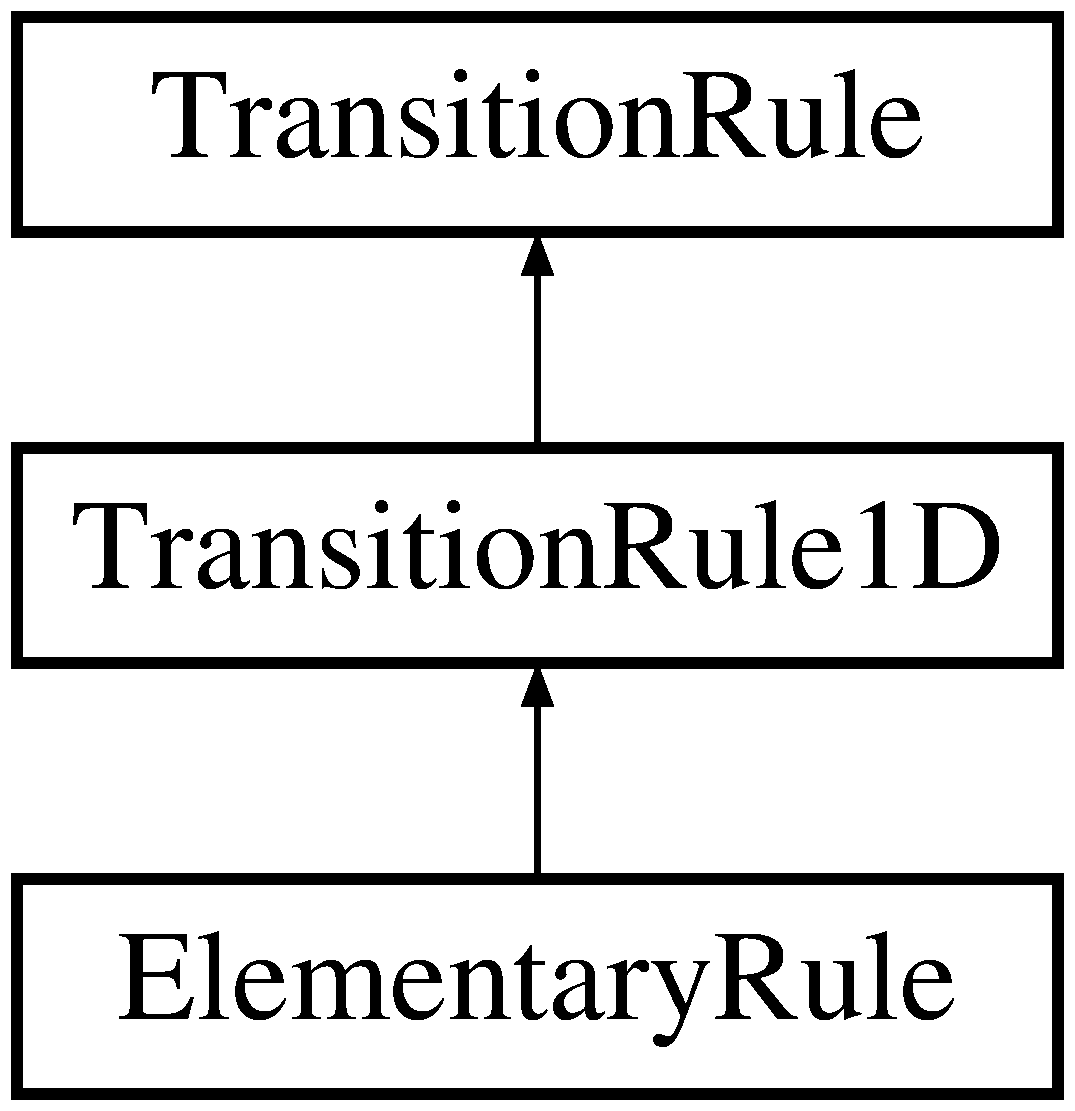
\includegraphics[height=3.000000cm]{class_elementary_rule}
\end{center}
\end{figure}
\subsection*{Public Member Functions}
\begin{DoxyCompactItemize}
\item 
\mbox{\Hypertarget{class_elementary_rule_a38451269153546c9d374f7f6df8cde6d}\label{class_elementary_rule_a38451269153546c9d374f7f6df8cde6d}} 
void {\bfseries Transition\+Cellule} (\mbox{\hyperlink{class_cell}{Cell}} const \&depart, \mbox{\hyperlink{class_cell}{Cell}} \&arrivee) const override
\item 
\mbox{\Hypertarget{class_elementary_rule_abcf6f8601c5ad393ee7e2a565e879f48}\label{class_elementary_rule_abcf6f8601c5ad393ee7e2a565e879f48}} 
{\bfseries Elementary\+Rule} (std\+::string rule, int nb\+Etats)
\end{DoxyCompactItemize}
\subsection*{Private Attributes}
\begin{DoxyCompactItemize}
\item 
\mbox{\Hypertarget{class_elementary_rule_a08733bd5dfc8395606006d513972f6c0}\label{class_elementary_rule_a08733bd5dfc8395606006d513972f6c0}} 
std\+::string {\bfseries m\+\_\+rule}
\item 
\mbox{\Hypertarget{class_elementary_rule_ade6ba3729cf8282c3b422a29b7c57a88}\label{class_elementary_rule_ade6ba3729cf8282c3b422a29b7c57a88}} 
int {\bfseries m\+\_\+nb\+Etats}
\end{DoxyCompactItemize}


The documentation for this class was generated from the following files\+:\begin{DoxyCompactItemize}
\item 
C\+:/\+Users/maxn0/git/\+L\+O21/\+Auto\+Cell/transitionrule.\+h\item 
C\+:/\+Users/maxn0/git/\+L\+O21/\+Auto\+Cell/transitionrule.\+cpp\end{DoxyCompactItemize}

\hypertarget{class_etat}{}\section{Etat Class Reference}
\label{class_etat}\index{Etat@{Etat}}
\subsection*{Public Member Functions}
\begin{DoxyCompactItemize}
\item 
\mbox{\Hypertarget{class_etat_a9de6f8f9bc1f9ec3296702a2ea9e7651}\label{class_etat_a9de6f8f9bc1f9ec3296702a2ea9e7651}} 
{\bfseries Etat} (int largeur, int longueur, \mbox{\hyperlink{class_generateur_etat}{Generateur\+Etat}} \&generateur, int nb\+Etats)
\item 
\mbox{\Hypertarget{class_etat_a4ab69207fc45fe1b193d3039eb456b32}\label{class_etat_a4ab69207fc45fe1b193d3039eb456b32}} 
{\bfseries Etat} (int largeur, int longueur, int $\ast$$\ast$tab)
\item 
\mbox{\Hypertarget{class_etat_a60fd78172b136c5011ccc840390ca378}\label{class_etat_a60fd78172b136c5011ccc840390ca378}} 
{\bfseries Etat} (int largeur, int longueur)
\item 
\mbox{\Hypertarget{class_etat_a6137bc65c74f615b6dca276ed1300e83}\label{class_etat_a6137bc65c74f615b6dca276ed1300e83}} 
{\bfseries Etat} (\mbox{\hyperlink{class_etat}{Etat}} const \&)=default
\item 
\mbox{\Hypertarget{class_etat_ad8cd3d55140d2b46784cb7623e998ee4}\label{class_etat_ad8cd3d55140d2b46784cb7623e998ee4}} 
void {\bfseries Regenerer} (int nb\+Etats)
\item 
\mbox{\Hypertarget{class_etat_a0ee4d5777ef97c1c7781e0e14b01699e}\label{class_etat_a0ee4d5777ef97c1c7781e0e14b01699e}} 
int {\bfseries Get\+Longueur} () const
\item 
\mbox{\Hypertarget{class_etat_a8dc404996c461e3cd4ebd301bfdcae4a}\label{class_etat_a8dc404996c461e3cd4ebd301bfdcae4a}} 
int {\bfseries Get\+Largeur} () const
\item 
\mbox{\Hypertarget{class_etat_a58c4c395d05101a68e8a28a8c1f769e9}\label{class_etat_a58c4c395d05101a68e8a28a8c1f769e9}} 
\mbox{\hyperlink{class_cell}{Cell}} const  \& {\bfseries Get\+Cellule} (int i, int j) const
\item 
\mbox{\Hypertarget{class_etat_addd390bbdb7b76148436a9a58c410f85}\label{class_etat_addd390bbdb7b76148436a9a58c410f85}} 
\mbox{\hyperlink{class_cell}{Cell}} \& {\bfseries Get\+Cellule} (int i, int j)
\item 
\mbox{\Hypertarget{class_etat_aeb0c23cfb166db846e567466dae0ebd1}\label{class_etat_aeb0c23cfb166db846e567466dae0ebd1}} 
void {\bfseries afficher} () const
\end{DoxyCompactItemize}
\subsection*{Private Attributes}
\begin{DoxyCompactItemize}
\item 
\mbox{\Hypertarget{class_etat_a914e5133fc90b6dc6b0bb31ea07aa1f0}\label{class_etat_a914e5133fc90b6dc6b0bb31ea07aa1f0}} 
\mbox{\hyperlink{class_generateur_etat}{Generateur\+Etat}} $\ast$ {\bfseries m\+\_\+generateur}
\item 
\mbox{\Hypertarget{class_etat_add8291e232f8219428147070f4126758}\label{class_etat_add8291e232f8219428147070f4126758}} 
std\+::vector$<$ std\+::vector$<$ \mbox{\hyperlink{class_cell}{Cell}} $>$ $>$ {\bfseries m\+\_\+cellules}
\item 
\mbox{\Hypertarget{class_etat_a2c443f1746c2e88a83ebeb15612aeea7}\label{class_etat_a2c443f1746c2e88a83ebeb15612aeea7}} 
int {\bfseries m\+\_\+longueur}
\item 
\mbox{\Hypertarget{class_etat_a227ad7e8e1bd5d692be7422444cb40d5}\label{class_etat_a227ad7e8e1bd5d692be7422444cb40d5}} 
int {\bfseries m\+\_\+largeur}
\end{DoxyCompactItemize}


The documentation for this class was generated from the following files\+:\begin{DoxyCompactItemize}
\item 
C\+:/\+Users/maxn0/git/\+L\+O21/\+Auto\+Cell/etat.\+h\item 
C\+:/\+Users/maxn0/git/\+L\+O21/\+Auto\+Cell/etat.\+cpp\end{DoxyCompactItemize}

\hypertarget{class_feu_foret}{}\section{Feu\+Foret Class Reference}
\label{class_feu_foret}\index{Feu\+Foret@{Feu\+Foret}}
Inheritance diagram for Feu\+Foret\+:\begin{figure}[H]
\begin{center}
\leavevmode
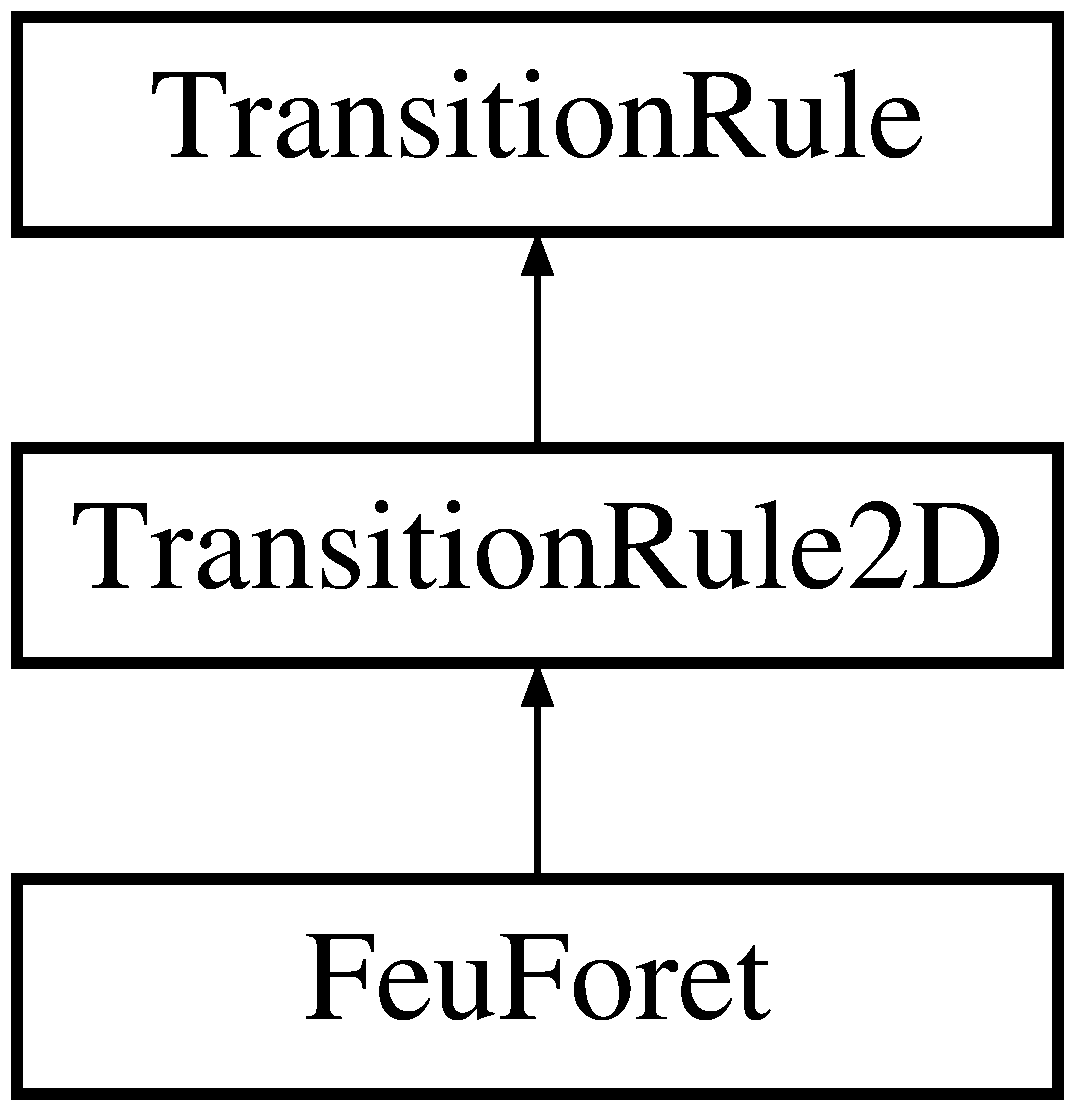
\includegraphics[height=3.000000cm]{class_feu_foret}
\end{center}
\end{figure}
\subsection*{Public Member Functions}
\begin{DoxyCompactItemize}
\item 
\mbox{\Hypertarget{class_feu_foret_a1fb3642690cc586faf0cbc6e9fae64cf}\label{class_feu_foret_a1fb3642690cc586faf0cbc6e9fae64cf}} 
void {\bfseries Transition\+Cellule} (\mbox{\hyperlink{class_cell}{Cell}} const \&depart, \mbox{\hyperlink{class_cell}{Cell}} \&arrivee) const override
\end{DoxyCompactItemize}


The documentation for this class was generated from the following files\+:\begin{DoxyCompactItemize}
\item 
C\+:/\+Users/maxn0/git/\+L\+O21/\+Auto\+Cell/transitionrule.\+h\item 
C\+:/\+Users/maxn0/git/\+L\+O21/\+Auto\+Cell/transitionrule.\+cpp\end{DoxyCompactItemize}

\hypertarget{class_game_of_life}{}\section{Référence de la classe Game\+Of\+Life}
\label{class_game_of_life}\index{Game\+Of\+Life@{Game\+Of\+Life}}


{\ttfamily \#include $<$transitionrule.\+h$>$}

Graphe d\textquotesingle{}héritage de Game\+Of\+Life\+:\begin{figure}[H]
\begin{center}
\leavevmode
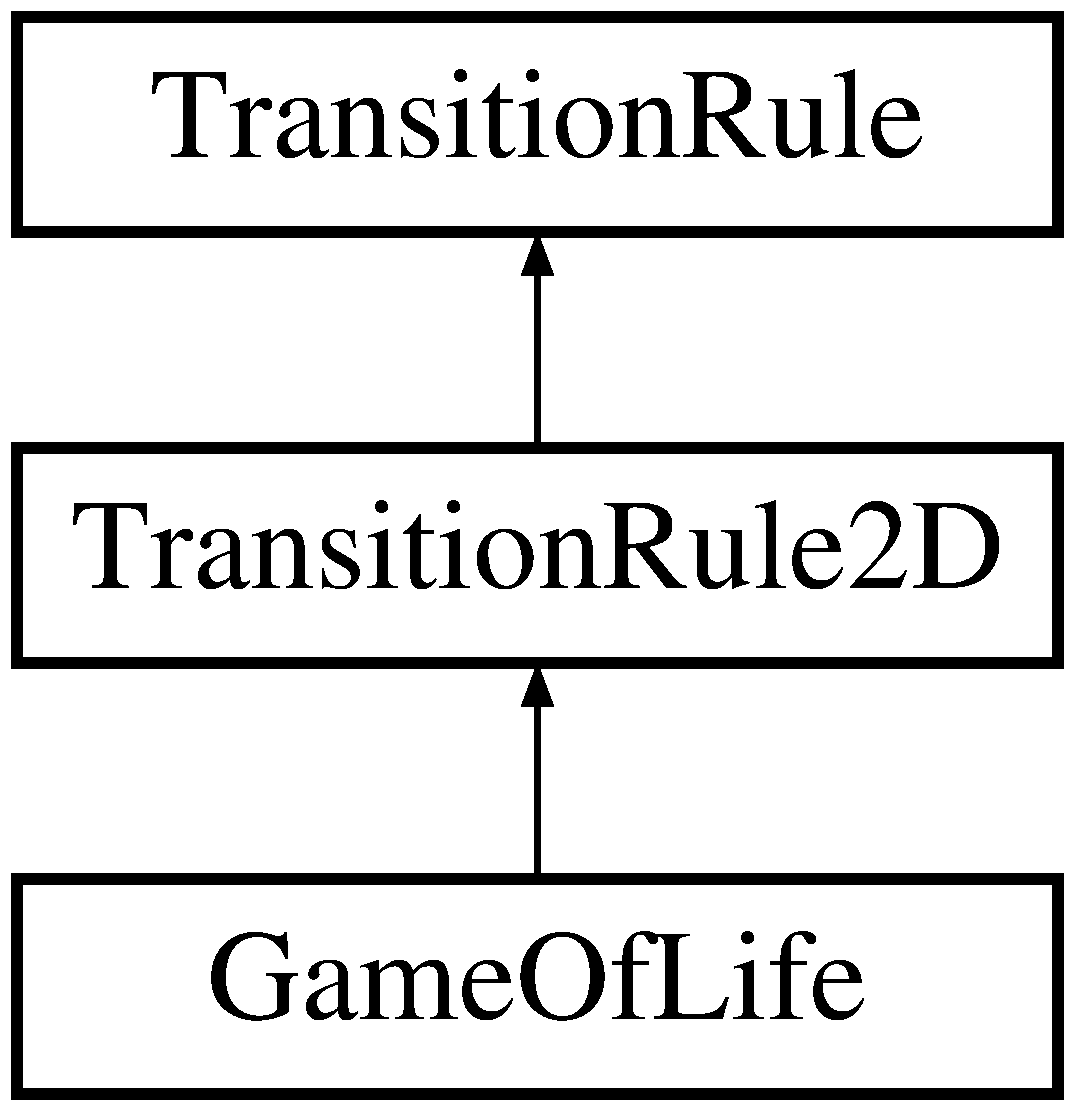
\includegraphics[height=2.000000cm]{class_game_of_life}
\end{center}
\end{figure}
\subsection*{Fonctions membres publiques}
\begin{DoxyCompactItemize}
\item 
void \mbox{\hyperlink{class_game_of_life_a12e6db1719e64adc023e1a7d2976d38d}{Transition\+Cellule}} (\mbox{\hyperlink{class_cell}{Cell}} const \&depart, \mbox{\hyperlink{class_cell}{Cell}} \&arrivee) const override
\item 
\mbox{\hyperlink{class_game_of_life_a033f778ad4b391bbf04dfa937f7b11df}{Game\+Of\+Life}} (unsigned int min\+Voisins\+Vivants, unsigned int max\+Voisins\+Vivants)
\item 
std\+::string \mbox{\hyperlink{class_game_of_life_a636421a27cb52e9f7ec161d141809919}{get\+Transition}} () const override
\item 
unsigned int \mbox{\hyperlink{class_game_of_life_afb8e0ee780b7e187266060cf9bec0578}{get\+Nb\+Etats}} () const
\item 
\mbox{\hyperlink{class_game_of_life_a3006eb8600b82f3deff3b8efe6725569}{$\sim$\+Game\+Of\+Life}} ()=default
\end{DoxyCompactItemize}
\subsection*{Attributs protégés}
\begin{DoxyCompactItemize}
\item 
unsigned int \mbox{\hyperlink{class_game_of_life_a851bf99201f554c12cdedf9fa227c321}{m\+\_\+min\+Voisins\+Vivants}}
\item 
unsigned int \mbox{\hyperlink{class_game_of_life_ad10ffab0e8d12ccac18ec5d4bd587fcc}{m\+\_\+max\+Voisins\+Vivants}}
\end{DoxyCompactItemize}


\subsection{Documentation des constructeurs et destructeur}
\mbox{\Hypertarget{class_game_of_life_a033f778ad4b391bbf04dfa937f7b11df}\label{class_game_of_life_a033f778ad4b391bbf04dfa937f7b11df}} 
\index{Game\+Of\+Life@{Game\+Of\+Life}!Game\+Of\+Life@{Game\+Of\+Life}}
\index{Game\+Of\+Life@{Game\+Of\+Life}!Game\+Of\+Life@{Game\+Of\+Life}}
\subsubsection{\texorpdfstring{Game\+Of\+Life()}{GameOfLife()}}
{\footnotesize\ttfamily Game\+Of\+Life\+::\+Game\+Of\+Life (\begin{DoxyParamCaption}\item[{unsigned int}]{min\+Voisins\+Vivants,  }\item[{unsigned int}]{max\+Voisins\+Vivants }\end{DoxyParamCaption})\hspace{0.3cm}{\ttfamily [inline]}}

\mbox{\Hypertarget{class_game_of_life_a3006eb8600b82f3deff3b8efe6725569}\label{class_game_of_life_a3006eb8600b82f3deff3b8efe6725569}} 
\index{Game\+Of\+Life@{Game\+Of\+Life}!````~Game\+Of\+Life@{$\sim$\+Game\+Of\+Life}}
\index{````~Game\+Of\+Life@{$\sim$\+Game\+Of\+Life}!Game\+Of\+Life@{Game\+Of\+Life}}
\subsubsection{\texorpdfstring{$\sim$\+Game\+Of\+Life()}{~GameOfLife()}}
{\footnotesize\ttfamily Game\+Of\+Life\+::$\sim$\+Game\+Of\+Life (\begin{DoxyParamCaption}{ }\end{DoxyParamCaption})\hspace{0.3cm}{\ttfamily [default]}}



\subsection{Documentation des fonctions membres}
\mbox{\Hypertarget{class_game_of_life_afb8e0ee780b7e187266060cf9bec0578}\label{class_game_of_life_afb8e0ee780b7e187266060cf9bec0578}} 
\index{Game\+Of\+Life@{Game\+Of\+Life}!get\+Nb\+Etats@{get\+Nb\+Etats}}
\index{get\+Nb\+Etats@{get\+Nb\+Etats}!Game\+Of\+Life@{Game\+Of\+Life}}
\subsubsection{\texorpdfstring{get\+Nb\+Etats()}{getNbEtats()}}
{\footnotesize\ttfamily unsigned int Game\+Of\+Life\+::get\+Nb\+Etats (\begin{DoxyParamCaption}{ }\end{DoxyParamCaption}) const\hspace{0.3cm}{\ttfamily [inline]}, {\ttfamily [virtual]}}



Implémente \mbox{\hyperlink{class_transition_rule_ad5bbcc6ef292bb079d8980f00d011a90}{Transition\+Rule}}.

\mbox{\Hypertarget{class_game_of_life_a636421a27cb52e9f7ec161d141809919}\label{class_game_of_life_a636421a27cb52e9f7ec161d141809919}} 
\index{Game\+Of\+Life@{Game\+Of\+Life}!get\+Transition@{get\+Transition}}
\index{get\+Transition@{get\+Transition}!Game\+Of\+Life@{Game\+Of\+Life}}
\subsubsection{\texorpdfstring{get\+Transition()}{getTransition()}}
{\footnotesize\ttfamily std\+::string Game\+Of\+Life\+::get\+Transition (\begin{DoxyParamCaption}{ }\end{DoxyParamCaption}) const\hspace{0.3cm}{\ttfamily [override]}, {\ttfamily [virtual]}}



Implémente \mbox{\hyperlink{class_transition_rule_af537bee6cca486c754ee94855242328c}{Transition\+Rule}}.

\mbox{\Hypertarget{class_game_of_life_a12e6db1719e64adc023e1a7d2976d38d}\label{class_game_of_life_a12e6db1719e64adc023e1a7d2976d38d}} 
\index{Game\+Of\+Life@{Game\+Of\+Life}!Transition\+Cellule@{Transition\+Cellule}}
\index{Transition\+Cellule@{Transition\+Cellule}!Game\+Of\+Life@{Game\+Of\+Life}}
\subsubsection{\texorpdfstring{Transition\+Cellule()}{TransitionCellule()}}
{\footnotesize\ttfamily void Game\+Of\+Life\+::\+Transition\+Cellule (\begin{DoxyParamCaption}\item[{\mbox{\hyperlink{class_cell}{Cell}} const \&}]{depart,  }\item[{\mbox{\hyperlink{class_cell}{Cell}} \&}]{arrivee }\end{DoxyParamCaption}) const\hspace{0.3cm}{\ttfamily [override]}, {\ttfamily [virtual]}}



Implémente \mbox{\hyperlink{class_transition_rule_a2b82a75ef494adc91b28755d55666e7a}{Transition\+Rule}}.



\subsection{Documentation des données membres}
\mbox{\Hypertarget{class_game_of_life_ad10ffab0e8d12ccac18ec5d4bd587fcc}\label{class_game_of_life_ad10ffab0e8d12ccac18ec5d4bd587fcc}} 
\index{Game\+Of\+Life@{Game\+Of\+Life}!m\+\_\+max\+Voisins\+Vivants@{m\+\_\+max\+Voisins\+Vivants}}
\index{m\+\_\+max\+Voisins\+Vivants@{m\+\_\+max\+Voisins\+Vivants}!Game\+Of\+Life@{Game\+Of\+Life}}
\subsubsection{\texorpdfstring{m\+\_\+max\+Voisins\+Vivants}{m\_maxVoisinsVivants}}
{\footnotesize\ttfamily unsigned int Game\+Of\+Life\+::m\+\_\+max\+Voisins\+Vivants\hspace{0.3cm}{\ttfamily [protected]}}

\mbox{\Hypertarget{class_game_of_life_a851bf99201f554c12cdedf9fa227c321}\label{class_game_of_life_a851bf99201f554c12cdedf9fa227c321}} 
\index{Game\+Of\+Life@{Game\+Of\+Life}!m\+\_\+min\+Voisins\+Vivants@{m\+\_\+min\+Voisins\+Vivants}}
\index{m\+\_\+min\+Voisins\+Vivants@{m\+\_\+min\+Voisins\+Vivants}!Game\+Of\+Life@{Game\+Of\+Life}}
\subsubsection{\texorpdfstring{m\+\_\+min\+Voisins\+Vivants}{m\_minVoisinsVivants}}
{\footnotesize\ttfamily unsigned int Game\+Of\+Life\+::m\+\_\+min\+Voisins\+Vivants\hspace{0.3cm}{\ttfamily [protected]}}



La documentation de cette classe a été générée à partir des fichiers suivants \+:\begin{DoxyCompactItemize}
\item 
C\+:/\+Users/maxn0/git/\+L\+O21/\+Auto\+Cell/\mbox{\hyperlink{transitionrule_8h}{transitionrule.\+h}}\item 
C\+:/\+Users/maxn0/git/\+L\+O21/\+Auto\+Cell/\mbox{\hyperlink{transitionrule_8cpp}{transitionrule.\+cpp}}\end{DoxyCompactItemize}

\hypertarget{class_generateur_etat}{}\section{Référence de la classe Generateur\+Etat}
\label{class_generateur_etat}\index{Generateur\+Etat@{Generateur\+Etat}}


{\ttfamily \#include $<$generateuretat.\+h$>$}

Graphe d\textquotesingle{}héritage de Generateur\+Etat\+:\begin{figure}[H]
\begin{center}
\leavevmode
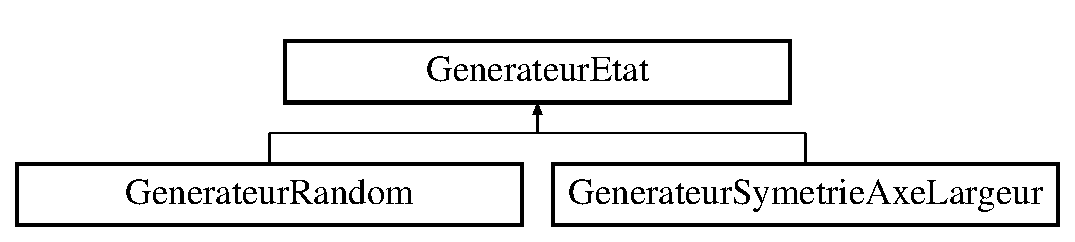
\includegraphics[height=2.000000cm]{class_generateur_etat}
\end{center}
\end{figure}
\subsection*{Fonctions membres publiques}
\begin{DoxyCompactItemize}
\item 
\mbox{\hyperlink{class_generateur_etat_a6ecebc169446d7f5fa40ed37af5abdaf}{Generateur\+Etat}} ()=default
\item 
virtual void \mbox{\hyperlink{class_generateur_etat_a0698d6706e0aaa2e597bdaf280806835}{Generer\+Etat}} (int nb\+Etats, \mbox{\hyperlink{class_etat}{Etat}} \&grille) const =0
\item 
virtual \mbox{\hyperlink{class_generateur_etat_a1ba21b5a12fa8855136363e338209d34}{$\sim$\+Generateur\+Etat}} ()=default
\end{DoxyCompactItemize}


\subsection{Documentation des constructeurs et destructeur}
\mbox{\Hypertarget{class_generateur_etat_a6ecebc169446d7f5fa40ed37af5abdaf}\label{class_generateur_etat_a6ecebc169446d7f5fa40ed37af5abdaf}} 
\index{Generateur\+Etat@{Generateur\+Etat}!Generateur\+Etat@{Generateur\+Etat}}
\index{Generateur\+Etat@{Generateur\+Etat}!Generateur\+Etat@{Generateur\+Etat}}
\subsubsection{\texorpdfstring{Generateur\+Etat()}{GenerateurEtat()}}
{\footnotesize\ttfamily Generateur\+Etat\+::\+Generateur\+Etat (\begin{DoxyParamCaption}{ }\end{DoxyParamCaption})\hspace{0.3cm}{\ttfamily [default]}}

\mbox{\Hypertarget{class_generateur_etat_a1ba21b5a12fa8855136363e338209d34}\label{class_generateur_etat_a1ba21b5a12fa8855136363e338209d34}} 
\index{Generateur\+Etat@{Generateur\+Etat}!````~Generateur\+Etat@{$\sim$\+Generateur\+Etat}}
\index{````~Generateur\+Etat@{$\sim$\+Generateur\+Etat}!Generateur\+Etat@{Generateur\+Etat}}
\subsubsection{\texorpdfstring{$\sim$\+Generateur\+Etat()}{~GenerateurEtat()}}
{\footnotesize\ttfamily virtual Generateur\+Etat\+::$\sim$\+Generateur\+Etat (\begin{DoxyParamCaption}{ }\end{DoxyParamCaption})\hspace{0.3cm}{\ttfamily [virtual]}, {\ttfamily [default]}}



\subsection{Documentation des fonctions membres}
\mbox{\Hypertarget{class_generateur_etat_a0698d6706e0aaa2e597bdaf280806835}\label{class_generateur_etat_a0698d6706e0aaa2e597bdaf280806835}} 
\index{Generateur\+Etat@{Generateur\+Etat}!Generer\+Etat@{Generer\+Etat}}
\index{Generer\+Etat@{Generer\+Etat}!Generateur\+Etat@{Generateur\+Etat}}
\subsubsection{\texorpdfstring{Generer\+Etat()}{GenererEtat()}}
{\footnotesize\ttfamily virtual void Generateur\+Etat\+::\+Generer\+Etat (\begin{DoxyParamCaption}\item[{int}]{nb\+Etats,  }\item[{\mbox{\hyperlink{class_etat}{Etat}} \&}]{grille }\end{DoxyParamCaption}) const\hspace{0.3cm}{\ttfamily [pure virtual]}}



Implémenté dans \mbox{\hyperlink{class_generateur_symetrie_axe_vertical_ae782046a73fc7624212c3c5988de949f}{Generateur\+Symetrie\+Axe\+Vertical}}, et \mbox{\hyperlink{class_generateur_random_ab110072502487c78f0b7dc0c7f2241c7}{Generateur\+Random}}.



La documentation de cette classe a été générée à partir du fichier suivant \+:\begin{DoxyCompactItemize}
\item 
C\+:/\+Users/maxn0/git/\+L\+O21/\+Auto\+Cell/\mbox{\hyperlink{generateuretat_8h}{generateuretat.\+h}}\end{DoxyCompactItemize}

\hypertarget{class_generateur_random}{}\section{Generateur\+Random Class Reference}
\label{class_generateur_random}\index{Generateur\+Random@{Generateur\+Random}}
Inheritance diagram for Generateur\+Random\+:\begin{figure}[H]
\begin{center}
\leavevmode
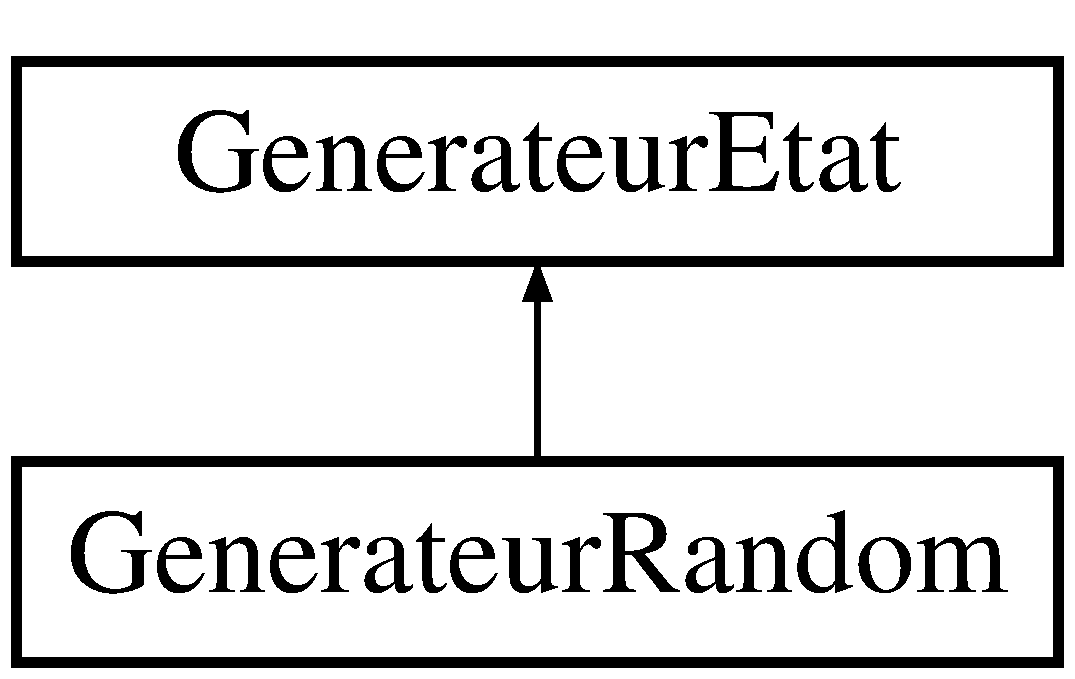
\includegraphics[height=2.000000cm]{class_generateur_random}
\end{center}
\end{figure}
\subsection*{Public Member Functions}
\begin{DoxyCompactItemize}
\item 
\mbox{\Hypertarget{class_generateur_random_ad6c15ee02504f5aa230068e5b1fa7a6b}\label{class_generateur_random_ad6c15ee02504f5aa230068e5b1fa7a6b}} 
void {\bfseries Generer\+Etat} (int nb\+Etat, std\+::vector$<$ std\+::vector$<$ \mbox{\hyperlink{class_cell}{Cell}} $>$$>$ \&tab) override
\end{DoxyCompactItemize}


The documentation for this class was generated from the following files\+:\begin{DoxyCompactItemize}
\item 
C\+:/\+Users/maxn0/git/\+L\+O21/\+Auto\+Cell/generateuretat.\+h\item 
C\+:/\+Users/maxn0/git/\+L\+O21/\+Auto\+Cell/generateuretat.\+cpp\end{DoxyCompactItemize}

\hypertarget{class_generateur_symetrie_axe_largeur}{}\section{Generateur\+Symetrie\+Axe\+Largeur Class Reference}
\label{class_generateur_symetrie_axe_largeur}\index{Generateur\+Symetrie\+Axe\+Largeur@{Generateur\+Symetrie\+Axe\+Largeur}}
Inheritance diagram for Generateur\+Symetrie\+Axe\+Largeur\+:\begin{figure}[H]
\begin{center}
\leavevmode
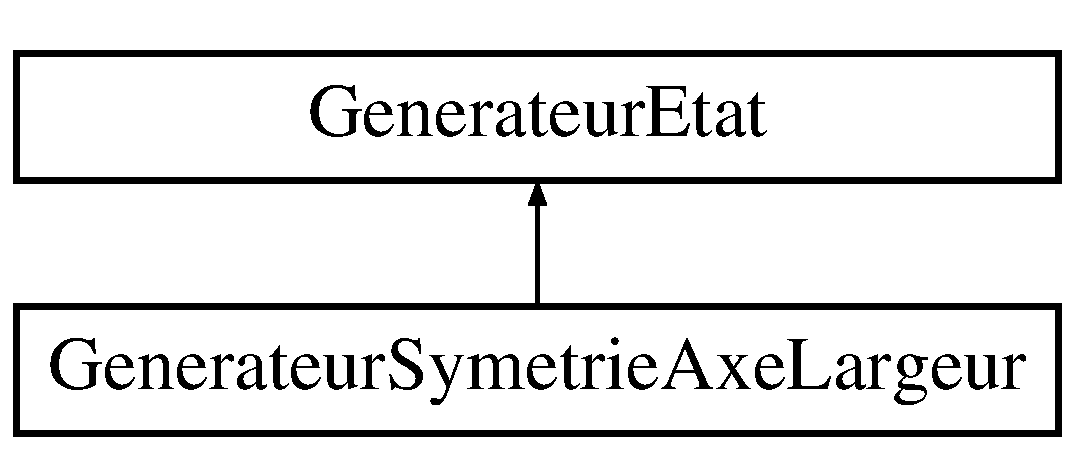
\includegraphics[height=2.000000cm]{class_generateur_symetrie_axe_largeur}
\end{center}
\end{figure}
\subsection*{Public Member Functions}
\begin{DoxyCompactItemize}
\item 
\mbox{\Hypertarget{class_generateur_symetrie_axe_largeur_ac11eee88b8728be13026ca408316561c}\label{class_generateur_symetrie_axe_largeur_ac11eee88b8728be13026ca408316561c}} 
void {\bfseries Generer\+Etat} (int nb\+Etat, std\+::vector$<$ std\+::vector$<$ \mbox{\hyperlink{class_cell}{Cell}} $>$$>$ \&tab) override
\end{DoxyCompactItemize}


The documentation for this class was generated from the following files\+:\begin{DoxyCompactItemize}
\item 
C\+:/\+Users/maxn0/git/\+L\+O21/\+Auto\+Cell/generateuretat.\+h\item 
C\+:/\+Users/maxn0/git/\+L\+O21/\+Auto\+Cell/generateuretat.\+cpp\end{DoxyCompactItemize}

\hypertarget{class_moore}{}\section{Référence de la classe Moore}
\label{class_moore}\index{Moore@{Moore}}


{\ttfamily \#include $<$voisinage.\+h$>$}

Graphe d\textquotesingle{}héritage de Moore\+:\begin{figure}[H]
\begin{center}
\leavevmode
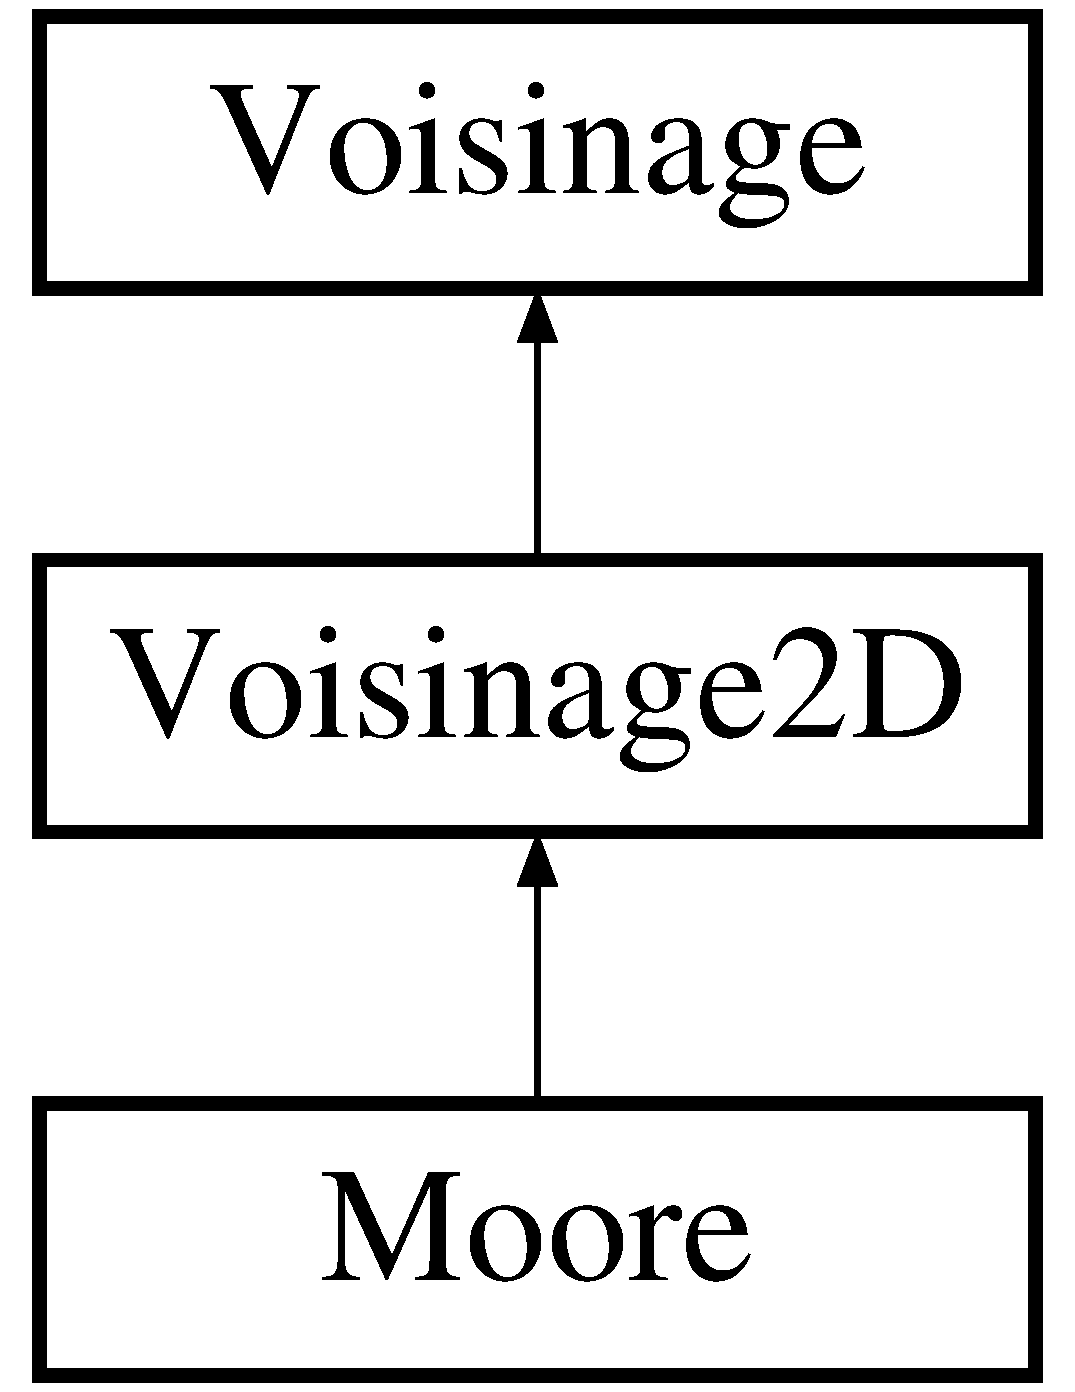
\includegraphics[height=2.000000cm]{class_moore}
\end{center}
\end{figure}
\subsection*{Fonctions membres publiques}
\begin{DoxyCompactItemize}
\item 
\mbox{\hyperlink{class_moore_a8b87d2d9c29ccbd0d8ed0081b4b58096}{Moore}} (int ordre)
\item 
\mbox{\hyperlink{class_moore_a18c2281db2524fff1559b5861cd2e3dc}{$\sim$\+Moore}} ()=default
\item 
void \mbox{\hyperlink{class_moore_a29a0a8f7b132429b5cbea4fdafcfd045}{definir\+Voisinage}} (\mbox{\hyperlink{class_etat}{Etat}} \&e) const override
\item 
std\+::string \mbox{\hyperlink{class_moore_af0398509c1540f611c000579714fbce7}{get\+Type}} () const
\end{DoxyCompactItemize}
\subsection*{Membres hérités additionnels}


\subsection{Documentation des constructeurs et destructeur}
\mbox{\Hypertarget{class_moore_a8b87d2d9c29ccbd0d8ed0081b4b58096}\label{class_moore_a8b87d2d9c29ccbd0d8ed0081b4b58096}} 
\index{Moore@{Moore}!Moore@{Moore}}
\index{Moore@{Moore}!Moore@{Moore}}
\subsubsection{\texorpdfstring{Moore()}{Moore()}}
{\footnotesize\ttfamily Moore\+::\+Moore (\begin{DoxyParamCaption}\item[{int}]{ordre }\end{DoxyParamCaption})\hspace{0.3cm}{\ttfamily [inline]}}

\mbox{\Hypertarget{class_moore_a18c2281db2524fff1559b5861cd2e3dc}\label{class_moore_a18c2281db2524fff1559b5861cd2e3dc}} 
\index{Moore@{Moore}!````~Moore@{$\sim$\+Moore}}
\index{````~Moore@{$\sim$\+Moore}!Moore@{Moore}}
\subsubsection{\texorpdfstring{$\sim$\+Moore()}{~Moore()}}
{\footnotesize\ttfamily Moore\+::$\sim$\+Moore (\begin{DoxyParamCaption}{ }\end{DoxyParamCaption})\hspace{0.3cm}{\ttfamily [default]}}



\subsection{Documentation des fonctions membres}
\mbox{\Hypertarget{class_moore_a29a0a8f7b132429b5cbea4fdafcfd045}\label{class_moore_a29a0a8f7b132429b5cbea4fdafcfd045}} 
\index{Moore@{Moore}!definir\+Voisinage@{definir\+Voisinage}}
\index{definir\+Voisinage@{definir\+Voisinage}!Moore@{Moore}}
\subsubsection{\texorpdfstring{definir\+Voisinage()}{definirVoisinage()}}
{\footnotesize\ttfamily void Moore\+::definir\+Voisinage (\begin{DoxyParamCaption}\item[{\mbox{\hyperlink{class_etat}{Etat}} \&}]{e }\end{DoxyParamCaption}) const\hspace{0.3cm}{\ttfamily [override]}, {\ttfamily [virtual]}}



Implémente \mbox{\hyperlink{class_voisinage_ac12f70bf8e971cbc8eaf8394de270d07}{Voisinage}}.

\mbox{\Hypertarget{class_moore_af0398509c1540f611c000579714fbce7}\label{class_moore_af0398509c1540f611c000579714fbce7}} 
\index{Moore@{Moore}!get\+Type@{get\+Type}}
\index{get\+Type@{get\+Type}!Moore@{Moore}}
\subsubsection{\texorpdfstring{get\+Type()}{getType()}}
{\footnotesize\ttfamily std\+::string Moore\+::get\+Type (\begin{DoxyParamCaption}{ }\end{DoxyParamCaption}) const\hspace{0.3cm}{\ttfamily [inline]}, {\ttfamily [virtual]}}



Implémente \mbox{\hyperlink{class_voisinage_a9853dfde1a68f5bb6333a8db001411a0}{Voisinage}}.



La documentation de cette classe a été générée à partir des fichiers suivants \+:\begin{DoxyCompactItemize}
\item 
C\+:/\+Users/maxn0/git/\+L\+O21/\+Auto\+Cell/\mbox{\hyperlink{voisinage_8h}{voisinage.\+h}}\item 
C\+:/\+Users/maxn0/git/\+L\+O21/\+Auto\+Cell/\mbox{\hyperlink{voisinage_8cpp}{voisinage.\+cpp}}\end{DoxyCompactItemize}

\hypertarget{class_transition_rule}{}\section{Transition\+Rule Class Reference}
\label{class_transition_rule}\index{Transition\+Rule@{Transition\+Rule}}
Inheritance diagram for Transition\+Rule\+:\begin{figure}[H]
\begin{center}
\leavevmode
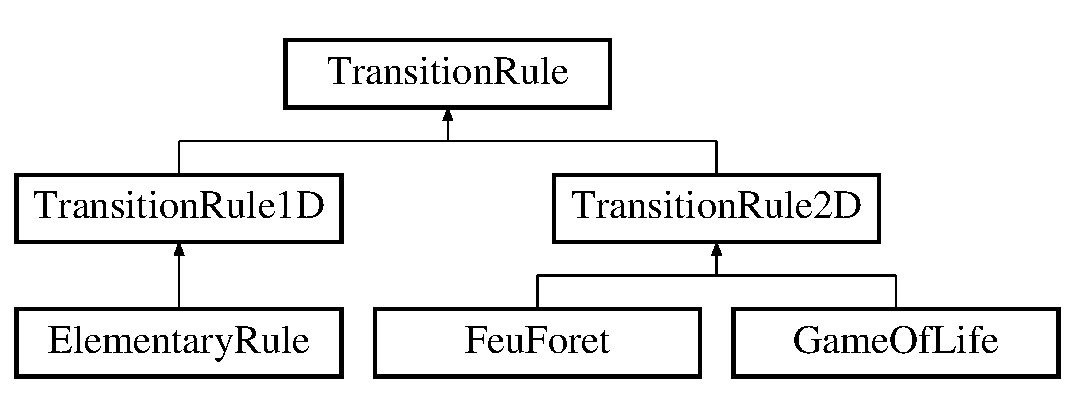
\includegraphics[height=3.000000cm]{class_transition_rule}
\end{center}
\end{figure}
\subsection*{Public Member Functions}
\begin{DoxyCompactItemize}
\item 
\mbox{\Hypertarget{class_transition_rule_a8570188a32e648ce3c08e76065f88fb7}\label{class_transition_rule_a8570188a32e648ce3c08e76065f88fb7}} 
virtual void {\bfseries Effectuer\+Transition} (\mbox{\hyperlink{class_etat}{Etat}} const \&depart, \mbox{\hyperlink{class_etat}{Etat}} \&arrivee) const
\item 
\mbox{\Hypertarget{class_transition_rule_a2b82a75ef494adc91b28755d55666e7a}\label{class_transition_rule_a2b82a75ef494adc91b28755d55666e7a}} 
virtual void {\bfseries Transition\+Cellule} (\mbox{\hyperlink{class_cell}{Cell}} const \&depart, \mbox{\hyperlink{class_cell}{Cell}} \&arrivee) const =0
\end{DoxyCompactItemize}


The documentation for this class was generated from the following files\+:\begin{DoxyCompactItemize}
\item 
C\+:/\+Users/maxn0/git/\+L\+O21/\+Auto\+Cell/transitionrule.\+h\item 
C\+:/\+Users/maxn0/git/\+L\+O21/\+Auto\+Cell/transitionrule.\+cpp\end{DoxyCompactItemize}

\hypertarget{class_transition_rule1_d}{}\section{Transition\+Rule1D Class Reference}
\label{class_transition_rule1_d}\index{Transition\+Rule1D@{Transition\+Rule1D}}
Inheritance diagram for Transition\+Rule1D\+:\begin{figure}[H]
\begin{center}
\leavevmode
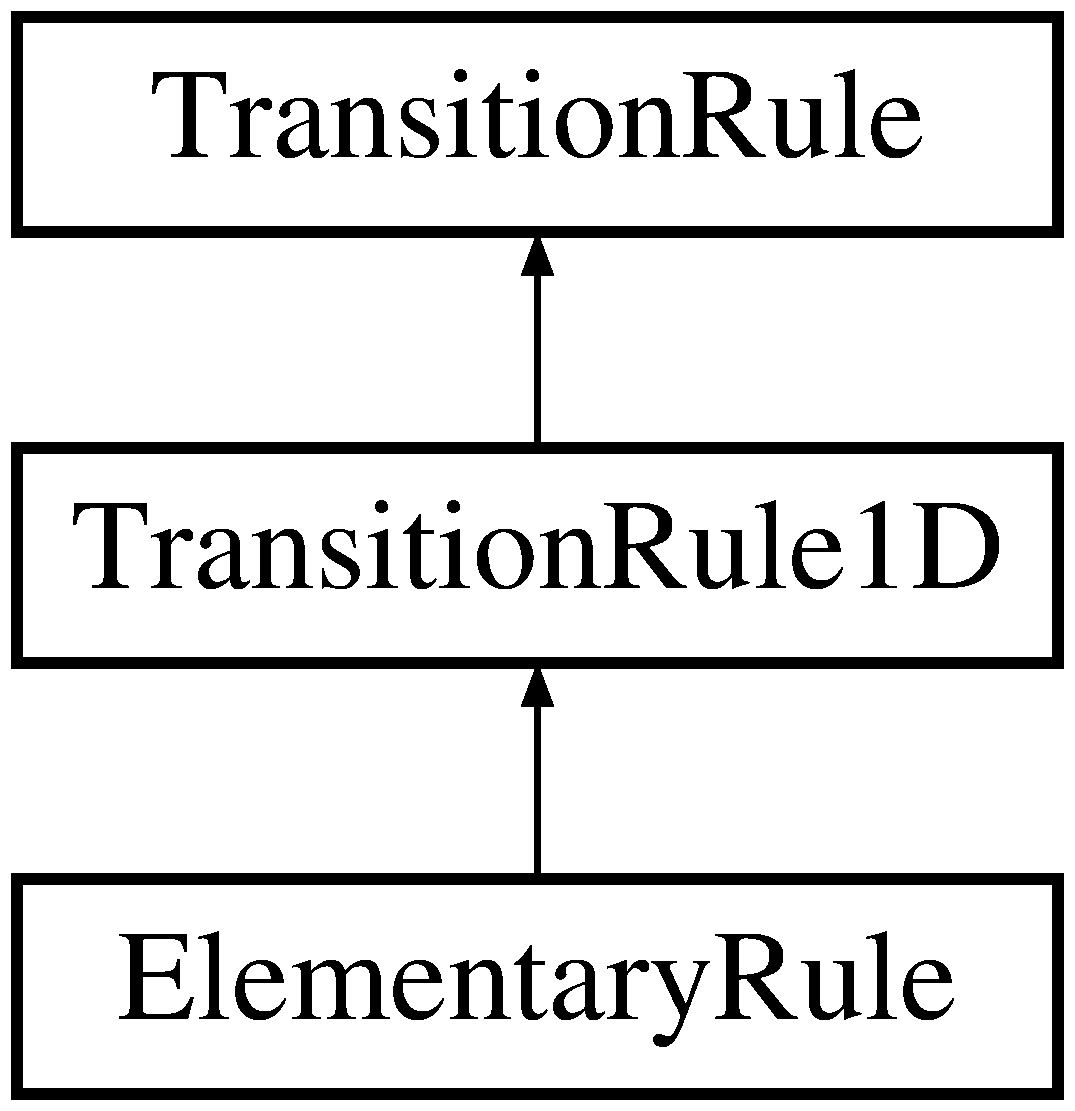
\includegraphics[height=3.000000cm]{class_transition_rule1_d}
\end{center}
\end{figure}
\subsection*{Additional Inherited Members}


The documentation for this class was generated from the following file\+:\begin{DoxyCompactItemize}
\item 
C\+:/\+Users/maxn0/git/\+L\+O21/\+Auto\+Cell/transitionrule.\+h\end{DoxyCompactItemize}

\hypertarget{class_transition_rule2_d}{}\section{Transition\+Rule2D Class Reference}
\label{class_transition_rule2_d}\index{Transition\+Rule2D@{Transition\+Rule2D}}
Inheritance diagram for Transition\+Rule2D\+:\begin{figure}[H]
\begin{center}
\leavevmode
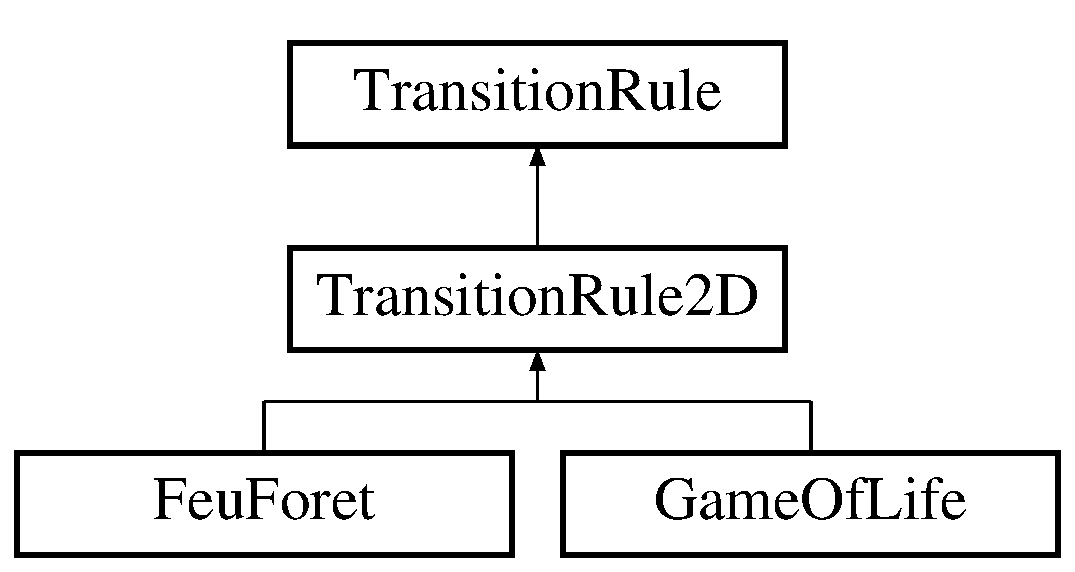
\includegraphics[height=3.000000cm]{class_transition_rule2_d}
\end{center}
\end{figure}
\subsection*{Additional Inherited Members}


The documentation for this class was generated from the following file\+:\begin{DoxyCompactItemize}
\item 
C\+:/\+Users/maxn0/git/\+L\+O21/\+Auto\+Cell/transitionrule.\+h\end{DoxyCompactItemize}

\hypertarget{class_voisinage}{}\section{Voisinage Class Reference}
\label{class_voisinage}\index{Voisinage@{Voisinage}}
Inheritance diagram for Voisinage\+:\begin{figure}[H]
\begin{center}
\leavevmode
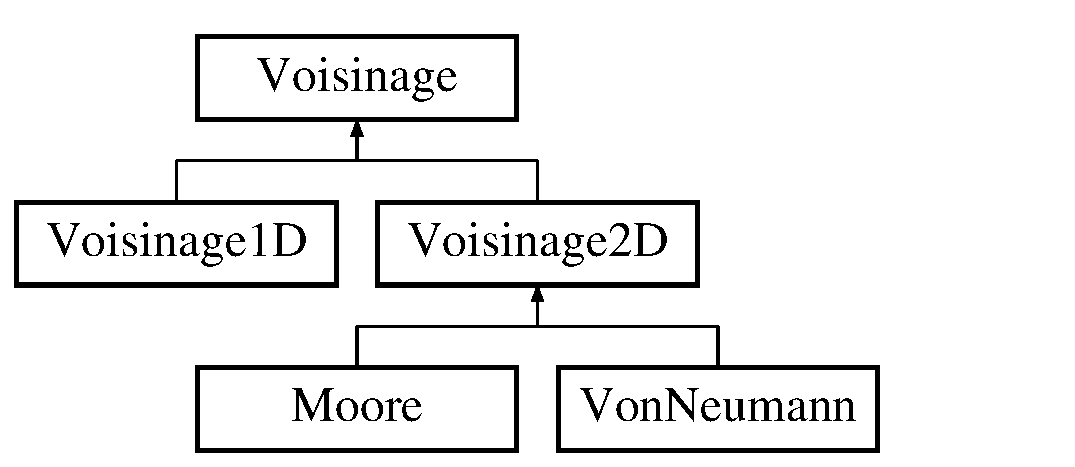
\includegraphics[height=3.000000cm]{class_voisinage}
\end{center}
\end{figure}
\subsection*{Public Member Functions}
\begin{DoxyCompactItemize}
\item 
\mbox{\Hypertarget{class_voisinage_a58416a610f5800ed165b0a68e9a78689}\label{class_voisinage_a58416a610f5800ed165b0a68e9a78689}} 
virtual void {\bfseries definir\+Voisinage} (\mbox{\hyperlink{class_etat}{Etat}} \&e, int ordre) const =0
\end{DoxyCompactItemize}


The documentation for this class was generated from the following file\+:\begin{DoxyCompactItemize}
\item 
C\+:/\+Users/maxn0/git/\+L\+O21/\+Auto\+Cell/voisinage.\+h\end{DoxyCompactItemize}

\hypertarget{class_voisinage1_d}{}\section{Référence de la classe Voisinage1D}
\label{class_voisinage1_d}\index{Voisinage1D@{Voisinage1D}}


{\ttfamily \#include $<$voisinage.\+h$>$}

Graphe d\textquotesingle{}héritage de Voisinage1D\+:\begin{figure}[H]
\begin{center}
\leavevmode
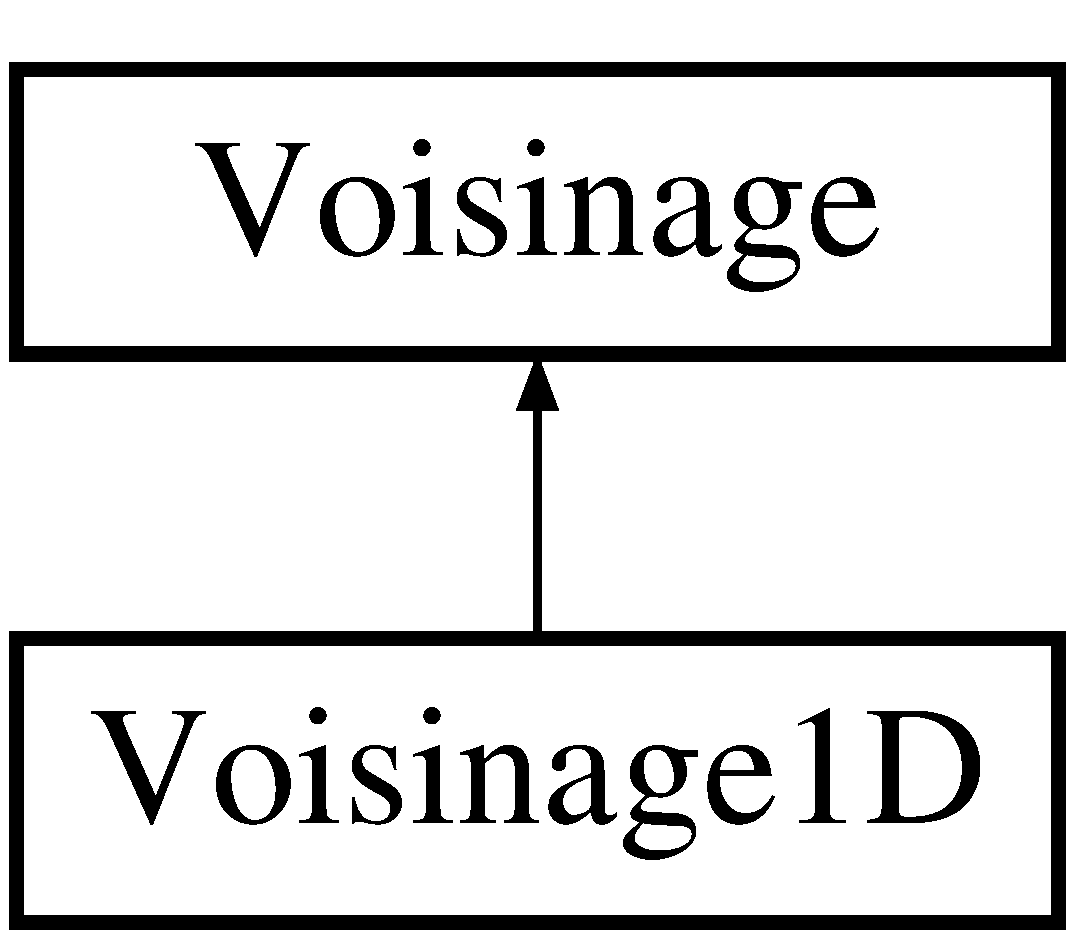
\includegraphics[height=2.000000cm]{class_voisinage1_d}
\end{center}
\end{figure}
\subsection*{Fonctions membres publiques}
\begin{DoxyCompactItemize}
\item 
\mbox{\hyperlink{class_voisinage1_d_a7077ba429224a21bc170dabcefea676e}{Voisinage1D}} (int ordre)
\item 
\mbox{\hyperlink{class_voisinage1_d_acb729fcae98b25a67d33098ef4a38260}{$\sim$\+Voisinage1D}} ()=default
\item 
void \mbox{\hyperlink{class_voisinage1_d_afdc267252af9b94fe26f5414d1472265}{definir\+Voisinage}} (\mbox{\hyperlink{class_etat}{Etat}} \&e) const final
\item 
std\+::string \mbox{\hyperlink{class_voisinage1_d_a92cc6dea76b6426d3cdaf849d18d205c}{get\+Type}} () const
\end{DoxyCompactItemize}
\subsection*{Membres hérités additionnels}


\subsection{Documentation des constructeurs et destructeur}
\mbox{\Hypertarget{class_voisinage1_d_a7077ba429224a21bc170dabcefea676e}\label{class_voisinage1_d_a7077ba429224a21bc170dabcefea676e}} 
\index{Voisinage1D@{Voisinage1D}!Voisinage1D@{Voisinage1D}}
\index{Voisinage1D@{Voisinage1D}!Voisinage1D@{Voisinage1D}}
\subsubsection{\texorpdfstring{Voisinage1\+D()}{Voisinage1D()}}
{\footnotesize\ttfamily Voisinage1\+D\+::\+Voisinage1D (\begin{DoxyParamCaption}\item[{int}]{ordre }\end{DoxyParamCaption})\hspace{0.3cm}{\ttfamily [inline]}}

\mbox{\Hypertarget{class_voisinage1_d_acb729fcae98b25a67d33098ef4a38260}\label{class_voisinage1_d_acb729fcae98b25a67d33098ef4a38260}} 
\index{Voisinage1D@{Voisinage1D}!````~Voisinage1D@{$\sim$\+Voisinage1D}}
\index{````~Voisinage1D@{$\sim$\+Voisinage1D}!Voisinage1D@{Voisinage1D}}
\subsubsection{\texorpdfstring{$\sim$\+Voisinage1\+D()}{~Voisinage1D()}}
{\footnotesize\ttfamily Voisinage1\+D\+::$\sim$\+Voisinage1D (\begin{DoxyParamCaption}{ }\end{DoxyParamCaption})\hspace{0.3cm}{\ttfamily [default]}}



\subsection{Documentation des fonctions membres}
\mbox{\Hypertarget{class_voisinage1_d_afdc267252af9b94fe26f5414d1472265}\label{class_voisinage1_d_afdc267252af9b94fe26f5414d1472265}} 
\index{Voisinage1D@{Voisinage1D}!definir\+Voisinage@{definir\+Voisinage}}
\index{definir\+Voisinage@{definir\+Voisinage}!Voisinage1D@{Voisinage1D}}
\subsubsection{\texorpdfstring{definir\+Voisinage()}{definirVoisinage()}}
{\footnotesize\ttfamily void Voisinage1\+D\+::definir\+Voisinage (\begin{DoxyParamCaption}\item[{\mbox{\hyperlink{class_etat}{Etat}} \&}]{e }\end{DoxyParamCaption}) const\hspace{0.3cm}{\ttfamily [final]}, {\ttfamily [virtual]}}



Implémente \mbox{\hyperlink{class_voisinage_ac12f70bf8e971cbc8eaf8394de270d07}{Voisinage}}.

\mbox{\Hypertarget{class_voisinage1_d_a92cc6dea76b6426d3cdaf849d18d205c}\label{class_voisinage1_d_a92cc6dea76b6426d3cdaf849d18d205c}} 
\index{Voisinage1D@{Voisinage1D}!get\+Type@{get\+Type}}
\index{get\+Type@{get\+Type}!Voisinage1D@{Voisinage1D}}
\subsubsection{\texorpdfstring{get\+Type()}{getType()}}
{\footnotesize\ttfamily std\+::string Voisinage1\+D\+::get\+Type (\begin{DoxyParamCaption}{ }\end{DoxyParamCaption}) const\hspace{0.3cm}{\ttfamily [inline]}, {\ttfamily [virtual]}}



Implémente \mbox{\hyperlink{class_voisinage_a9853dfde1a68f5bb6333a8db001411a0}{Voisinage}}.



La documentation de cette classe a été générée à partir des fichiers suivants \+:\begin{DoxyCompactItemize}
\item 
C\+:/\+Users/maxn0/git/\+L\+O21/\+Auto\+Cell/\mbox{\hyperlink{voisinage_8h}{voisinage.\+h}}\item 
C\+:/\+Users/maxn0/git/\+L\+O21/\+Auto\+Cell/\mbox{\hyperlink{voisinage_8cpp}{voisinage.\+cpp}}\end{DoxyCompactItemize}

\hypertarget{class_voisinage2_d}{}\section{Voisinage2D Class Reference}
\label{class_voisinage2_d}\index{Voisinage2D@{Voisinage2D}}
Inheritance diagram for Voisinage2D\+:\begin{figure}[H]
\begin{center}
\leavevmode
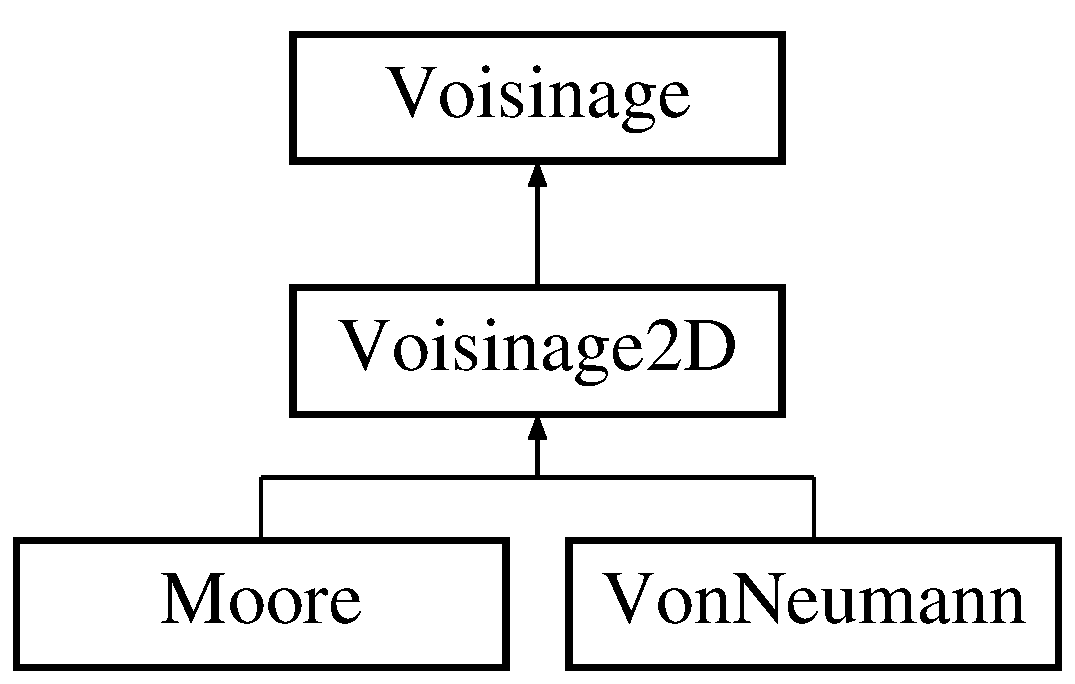
\includegraphics[height=3.000000cm]{class_voisinage2_d}
\end{center}
\end{figure}
\subsection*{Additional Inherited Members}


The documentation for this class was generated from the following file\+:\begin{DoxyCompactItemize}
\item 
C\+:/\+Users/maxn0/git/\+L\+O21/\+Auto\+Cell/voisinage.\+h\end{DoxyCompactItemize}

\hypertarget{class_von_neumann}{}\section{Von\+Neumann Class Reference}
\label{class_von_neumann}\index{Von\+Neumann@{Von\+Neumann}}
Inheritance diagram for Von\+Neumann\+:\begin{figure}[H]
\begin{center}
\leavevmode
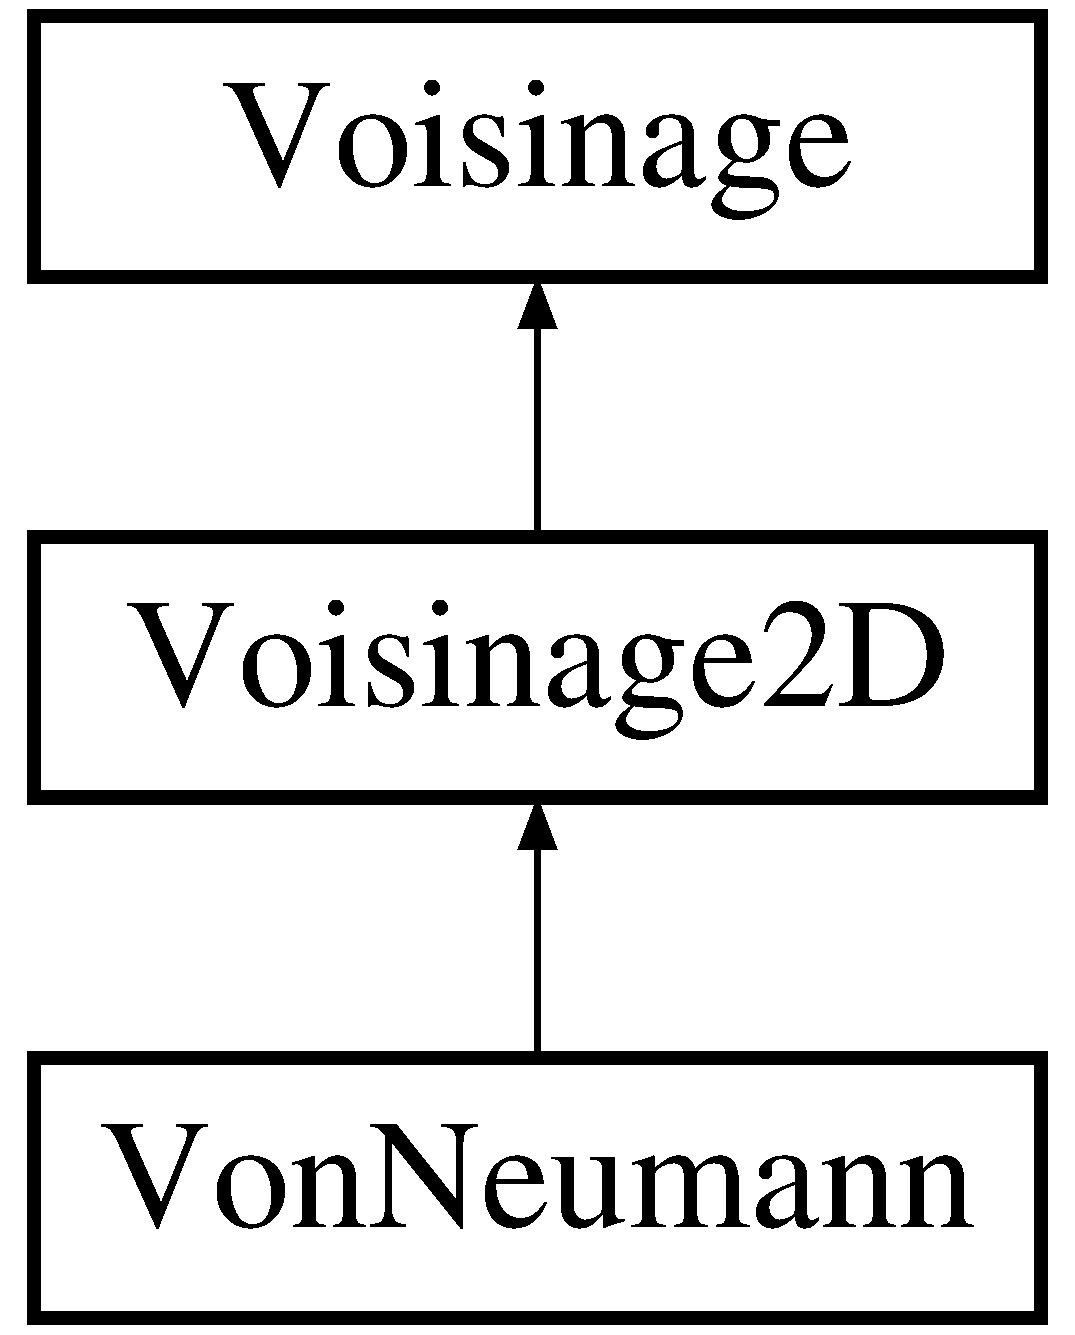
\includegraphics[height=3.000000cm]{class_von_neumann}
\end{center}
\end{figure}
\subsection*{Public Member Functions}
\begin{DoxyCompactItemize}
\item 
\mbox{\Hypertarget{class_von_neumann_a20b458d41f227a3d39f44e08376b80eb}\label{class_von_neumann_a20b458d41f227a3d39f44e08376b80eb}} 
void {\bfseries definir\+Voisinage} (\mbox{\hyperlink{class_etat}{Etat}} \&e, int ordre) const override
\end{DoxyCompactItemize}


The documentation for this class was generated from the following files\+:\begin{DoxyCompactItemize}
\item 
C\+:/\+Users/maxn0/git/\+L\+O21/\+Auto\+Cell/voisinage.\+h\item 
C\+:/\+Users/maxn0/git/\+L\+O21/\+Auto\+Cell/voisinage.\+cpp\end{DoxyCompactItemize}

%--- End generated contents ---

% Index
\backmatter
\newpage
\phantomsection
\clearemptydoublepage
\addcontentsline{toc}{chapter}{Index}
\printindex

\end{document}
